%!TEX root = ../gronskiy_phd_thesis.tex 
\chapter[Approximation-Based Regularization for Robust Optimization]{Approximation-Based Regularization \\ for Robust Optimization}
\label{ch:gen_appch}

\hfill
\begin{minipage}[t]{.75\textwidth}
\textit{``Truth is much too complicated to allow anything but approximations.''} \\
  \hrule
  \vspace{.2cm}
  \hfill
  \textsc{--- John von NEUMANN}, ``The Mathematician''
\end{minipage}

\section{Introduction}

\subsection{Motivation}

Within a given data set, not all information is useful~--- given measurement
error, some part of it explains noise, not the true functional dependencies.
Hence, there exists an inevitable limitation on the amount of information bits
one should use in order to avoid overfitting. However, another curse~---
underfitting~--- happens if for some reason the solver decides to play on the
safe side and uses less information than would be optimal. We refer to this
phenomenon as the \textit{informativeness vs. robustness trade-off}.
\index{Underfitting}

In the line of research started
by~\citet{conf/isit/Buhmann10,conf/mcpr2/Buhmann11}, an approach of utilizing
self-calibrating\footnote{Sometimes ``self-calibrating'' is replaced by
``context-sensitive''.} optimization procedures is devised and advocated. In its
essential part, this approach aims at maximizing (through a set of tools
discussed below) the amount of useful information, thereby making 
solutions both statistically robust \textit{and} informative.

This approach features~\citep[cf.][]{Busetto:PhD,jcss:2017}, among others, the following key
properties: 
\begin{itemize}
  \item it does not require any knowledge on
    probability distributions of input instances, particularly not whether the
    noise is systematic or random;
  \item it allows to quantify the quality of the obtained solution w.r.t.~ 
    unseen data instances;
  \item moreover, it makes possible to rank different models.
\end{itemize}

In this chapter, we will provide justification of this approach, as well as
introduce some prototypic examples proving its usability. We will also discuss
possible generalizations and adjustments of this approach, which will be
addressed in the next chapters.

\subsection{Contributions and Outline of the Chapter}
\label{sec:asc_contribs}

As main contributions of this chapter, we
\begin{itemize}
  \item provide a justification and revisit the approach for robust optimization
    called Approximation Set Coding;\index{ASC|see{Approximation Set Coding}} \index{Approximation Set Coding}
  \item introduce and evaluate the simplest, yet interpretable proof-of-concept
    model which shows experimentally the superiority of the ASC-based approach
    and refers to clear intuitions about the mechanism thereof;
  \item prove a theoretical result which suggests one step further in the direction
    of eliminating the computational bottleneck of the ASC~--- computing the ASC
    score;
  \item introduce a so-called Gibbs relaxation of the ASC approach, give 
    a rationale behind it and experimentally evaluate its performance.
\end{itemize}

The chapter is outlined as follows. First, a background and related work are
given in Section~\ref{sec:gen_appch_related_work}. We then provide technical
preliminaries (setting and model assumptions) in
Section~\ref{sec:gen_appch_setting_and_model}. A comprehensive introduction into
the original approximation set-based approach is then given in
Section~\ref{sec:asc_original}. Section~\ref{sec:similarity_approach_intro}
presents an analogical approach to robust optimization. We then give a
proof-of-concept experimental confirmation of the validity of approximation
set-based methods in Section~\ref{sec:proof_of_concept}. Further, we address one
problem which is very characteristic bottleneck for the most of applications of
approximation set-based approaches and solve it in
Section~\ref{sec:analytic_solution}. We then explain how a relaxation of the
approach (called Gibbs relaxation) works in Section~\ref{sec:gibbs_relaxation_of_sim}
and show experimental results for it. Finally, concluding remarks follow
in~Section~\ref{sec:gen_appch_conclusion}.

\myremark Section~\ref{sec:similarity_approach_intro} is included into the
thesis for the sake of ``self-containedness'', and presents an approach not due
to the author of this thesis. For smooth integration into this thesis, we
provided necessary terminological and notational adaptation, but
nevertheless, some small parts of the text of
Section~\ref{sec:similarity_approach_intro}, as well as
Section~\ref{sec:gen_appch_conclusion} may still be similar to that
of~\citet{Sramek:PhD}. Sections~\ref{sec:proof_of_concept},~\ref{sec:analytic_solution}
and~\ref{sec:gibbs_relaxation_of_sim} are a result of joint work hence their
textual presentation may be partially similar to that of~\citet{jcss:2017}.

\section{Background and Related Work Overview}
\label{sec:gen_appch_related_work}

When dealing with uncertain (noisy) inputs, the model designer always confronts
with two related questions:
\begin{itemize}
  \item For a given model, how to provide a well-generalizing regularization?
  \item For a predefined set of models, how to establish an ordering of them which
  would reflect their generalization capability?
\end{itemize}

While we introduce an approach which solves both tasks, in this chapter we will
mainly concentrate on the first application of it, while the next chapter
(Chapter~\ref{ch:mst}) addresses the second one. For now, however, we summarize
an overview of both tasks.

\subsection{Generalization and Stability in Learning}
\label{sec:generalization_stability_in_learning}
When dealing with noisy inputs, a designer of an empirical risk minimization
(ERM) algorithm is always confronting with how well the learned solution
generalizes to the unknown test sets. In fact, the whole field of statistical
learning theory~\citep{Vapnik71,Vapnik:1982} \index{Statistical
learning theory} has been in its core posing this
questions since 70s of the last century. It focuses on the question: for a given
algorithm, can we derive bounds of its generalization error~\citep{Bishop:2006}?
\index{ERM|see{Empirical Risk Minimization}} 
\index{Empirical Risk Minimization} 

The ways of bounding generalization error \index{Generalization error} can be, in our view, split into
three\footnote{These classes are very much interrelated. We brought such
classification for simplicity and don't pretend it to be the only division
possible.} classes: to a more classical one belongs, e.g.~bounding
generalization error via considering properties of \textit{hypothesis space}
such as VC-dimension~\citep{Vapnik71,Vapnik:1982} or Rademacher
complexity~\citep{Shalev-Shwartz:2014}.

Another class of research directions encompasses approaches where one derives
such bounds using the so-called (hypothesis, error or uniform)
stability~\citep{Devroye79,Bousquet:2002} property of the ERM algorithm, which,
in essence, reflects how critical are the fluctuations of the input data for the
outcome of an algorithm. As a side remark, we can note that from the technical
standpoint, the mentioned bounds utilized various concentration
inequalities~\citep{RaginskyS15}. 

Lastly, stability \index{Stability} (and thus generalization) properties have recently enjoyed
research from the information theoretic prospective, considering a learning
algorithm as a channel from the input to output~\citep{Russo15,Xu17} and
relating stability to the mutual information between the input and the output.
To the advantages of this third class of approaches belongs the fact, that the
bounds provided by it, involve \textit{both} the properties of the hypothesis
space and the learning algorithm (as opposed to the aforementioned methods). To
the same ``information theory-inspired'' class can we assign a recent work
by~\citet{Alabdulmohsin:2015} which relates generalization to a total variation
\index{Total variation information} information.

\myremark The approach via input-output mutual information comes very close to
the one introduced and advocated in this chapter. However, we should note that
both approaches stem from different definitions of the communication channel
used to derive error bounds.

\myremark It should be noted here that all the above methods only provide ways 
to guarantee certain performance when the learning algorithm is fixed. They do
not answer the question how to regularize its solutions for a more robust
performance. In contrast, the approach presented and tested in this chapter does
exactly this.

\subsection{Model Selection}
Besides quantifying the quality of a given ERM solution (overview for which was
given above), a modeler can ask another question: how to choose between two
possible models, taking into account various properties such as e.g.~complexity?
A long line research which addressed this question is presented by methods such
as the Minimum Description Length (MDL) principle~\citep{Rissanen:1978}, the
Akaike Information Criterion (AIC), the Bayesian Information Criterion (BIC) or
the Generalized Information Criterion~\citep[for an overview,
see][]{Konishi:2007}.
\index{Model validation}
\index{Model validation!MDL}
\index{Model validation!AIC}
\index{Model validation!BIC}
\index{AIC|see{Model validation}}
\index{BIC|see{Model validation}}
\index{MDL|see{Model validation}}

\subsection{Robust Optimization}

Besides the approaches characteristic for statistical learning theory, there
exists a methodological direction called \textit{robust optimization}.
\index{Robust optimization}
%
Being very close to the approaches above, robust optimization deals with models
for the uncertain input~--- however, contrary to the approaches traditional for
statistical learning theory, in the field of robust optimization, it is
explicitly discouraged to assume the knowledge of the input data distribution,
although some information (for example, if the data comes form certain interval
domain or not) might be available.
%
For a comprehensive overview of robust optimization approaches, we recommend a
recent survey by~\citet{series/lncs/GoerigkS16}.

The closest point of contact between the robust optimization approaches and
approaches of the above Section~\ref{sec:generalization_stability_in_learning}
is, in out view, \textit{optimization for stable inputs} which makes an attempt
to understand the connection between fluctuations of the input and the output,
i.e. some sort of stability~\citep{journals/cpc/BiluL12,%
conf/sirocco/BiloGGPW09,journals/scheduling/GattoW11,conf/sofsem/MihalakSSW11}.



% \section{Related Work}
% \label{sec:gen_appch_related_work}
% ­Noisy inputs received attention in a variety of ways. \emph{Stochatic
% programming}~\cite{Schneider07,KallM05} utilizes random variables to model
% uncertainty in the input data. When the random variables are used only in the
% optimization method and not in modelling the problem, one commonly refers to
% \emph{stochastic optimization}. Stochastic methods often aim at minimizing or
% maximizing the expected cost, and in general they assume all probability
% distributions to be known exactly. However, this is quite a strong assumption
% because as argued earlier, the patterns behind real-world noise might be complex
% and not easily observable.

% \paragraph{Sensitivity analysis and stability}

% \emph{Robust optimization}~\cite{BenTalEGN09} assumes that we are given a set of
% so-called scenarios instead of a probability distribution over the possible
% input instances. Each scenario corresponds to one particular realization of the
% input. Strict robustness computes a solution that is feasible in every scenario,
% and that minimizes the maximum cost over all scenarios. Instead of minimizing
% the maximum absolute cost, min-max regret robustness~\cite{journals/asa/Savage51}
% minimizes the largest regret (i.e., the difference between the cost of the
% chosen solution and the cost of the minimum in the given scenario) over all
% scenarios. However, a worst case perspective in which an adversary will reveal
% the worst possible instance, given the chosen solution, is far too pessimistic
% for real-world applications. Therefore, various relaxations of the
% aforementioned robust optimization approaches have been
% proposed~\cite{series/lncs/GoerigkS16}. For example, cardinality constrained
% robustness~\cite{journals/ior/BertsimasS04} allows a certain amount of problem
% constraints to be violated, while light robustness~\cite{journals/mmor/Schobel14}
% allows to relax the constraints. The disadvantage of these approaches is that
% they might compute solutions that are no longer feasible for the actual
% scenario. To guarantee feasibility in all cases, recoverable robust
% optimization~\cite{series/lncs/LiebchenLMS09} goes one step further and allows
% the proposed solution to be modified after the true instance (or parts of it)
% have been revealed. For an overview on robust optimization approaches, we refer
% to a recent survey by Goerigk and Sch\"obel~\cite{series/lncs/GoerigkS16}.

% \emph{Optimization for stable inputs} attempts to understand when and how small
% changes in the input data affect the solution~\cite{journals/cpc/BiluL12,%
% conf/sirocco/BiloGGPW09,journals/scheduling/GattoW11,conf/sofsem/MihalakSSW11}.
% %
% % \emph{Info-gap decision theory} is peculiar in that it models uncertainty as an
% % information gap rather than a probability~\cite{BenHaim06}.
% % \tptodo{Elaborate or remove}
% % %
% Optimization for sample average~\cite{KleywegtSH02} aims at solving optimization
% problems preceded by averaging several inputs into one.


\section{Setting and Generative Model Assumptions}
\label{sec:gen_appch_setting_and_model}

\subsection{Optimization Problem}
\label{sec:optimization_problem_description}

In the setting we are going to analyze in this and the next chapters, the
following components are assumed to be defined: 

\begin{itemize}
  \item A set $\mathcal{X}$ of possible \textit{data instances} $X$:
  \begin{equation}
    \mathcal{X} \ni X,
  \end{equation}
  \nomenclature[A, 01]{$\mathcal{X}$}{source of data instances}%
  \nomenclature[A, 01a]{$X \in \mathcal{X}$}{[random] data instance}%
  on which no further assumptions (e.g. structure, finiteness, countability) are
  imposed in the most general case (see below in
  Section~\ref{sec:data_generation_model} for possible specifications of such
  assumptions).
  \index{Data instance}

  \item A set $\mathcal{C}$ of possible \textit{solutions}, or
  \textit{hypotheses} $c$:
  \begin{equation}
    \mathcal{C} \ni c,
  \end{equation}
  \nomenclature[A, 01b]{$\mathcal{C}$}{set of solutions}%
  \nomenclature[A, 01c]{$c \in \mathcal{C}$}{solution}% can add \nomnorefeq
  where again no further structural or finiteness assumptions are imposed.

  \item An \textit{objective function} $R(c, X)$ representing the value of a
  given solution solution $c$ for a data instance $X$:
  \begin{equation}\label{eq:cost_function}
    R(c, X) \colon \mathcal{C} \times \mathcal{X} \to \mathbb{R}.
  \end{equation}
  \nomenclature[A, 01d]{$R(c, X)$}{cost function}%
  If not stated otherwise, we will assume a minimization (i.e. ``cost'', ``error''
  or ``energy'') semantics of $R(c,X)$ and call it a \textit{cost function}.
\end{itemize}

\begin{definition}\label{def:optimization_problem_definition}
  Provided that a \textit{solution feasibility} assumption is fulfilled, i.e.~any
  solution $c \in \mathcal{C}$ is \textit{feasible} (i.e.~valid) for any data
  instance $X \in \mathcal{X}$, then we can say that these three components define a
  valid \textit{optimization problem} denoted by a triplet $\mathcal{P} =
  (\mathcal{X}, \mathcal{C}, R)$.
  \nomenclature[A, 01e]{$\mathcal{P} = (\mathcal{X}, \mathcal{C}, R)$}{optimization problem \nomnorefeqpage\hfill Def.~\ref{def:optimization_problem_definition}}%
  \index{Optimization problem}
\end{definition}

The optimization goal consists in finding the
set of those solutions which minimize the cost function:
\begin{equation}
  \mathcal{C}^\bot(X) \coloneqq \arg \min_{c \in \mathcal{C}} R(c, X).
\end{equation}
\nomenclature[A, 01f]{$\mathcal{C}^\bot(X)$}{set of empirical optimizers}%
With a bit of notation abuse we will also write
\begin{equation}
  c^\bot(X) \coloneqq \arg \min_{c \in \mathcal{C}} R(c, X) \in \mathcal{C}^\bot(X),
\end{equation}
\index{Global minimizer}
meaning a \textit{one} (out of many possible) optimal solution (global
minimizer). We will denote the optimal cost as:
\begin{equation}
  R^\bot(X) \coloneqq  \min_{c \in \mathcal{C}} R(c, X).
\end{equation}
\nomenclature[A, 01g]{$R^\bot(X)$}{optimal cost}%

\subsection{Data Generation Model}
\label{sec:data_generation_model}

Dealing with \textit{uncertainty} in optimization requires to define a data
generation process.

In the following, we will simply assume that there is exists \textit{true
(ground, signal) data instance} $X^0$, from which the \textit{noise-contaminated
data instances} are obtained independently, i.e.:
\begin{equation}\label{eq:data_gen_model}
  X', X'', X''', \dots \sim PG(X | X^0)
\end{equation}
through a \textit{problem generating} process $PG(\cdot | X^0)$. 
\nomenclature[A, 01h]{$PG(X \mid X^0)$}{problem generator}%
\index{Problem generator}
Note that the problem generating process is parametrized through the ground
truth $X^0$. Note also that the obtained data instances are independent,
conditioned on the $X^0$:
\begin{equation}\label{eq:pg_independence}
  \text{for any data instances $X', X'' \sim PG(X | X^0)$:\quad } X'
  \independent X'' | X^0.
\end{equation}  
\index{Data instance!Ground truth}

\myremark Although this notation might seem complex, it is actually very
straightforward. In most cases we consider, $X \in \mathcal{X}$ will be just a
vector of random (generated by $PG(\cdot)$) weights from which the costs $R(c,
X)$ are constructed.

\section{Approximation Set-Based Approach}
\label{sec:asc_original}

\index{Approximation Set Coding}
In this section, we will introduce the notions related to Approximation Set
Coding framework~--- a successful way of regularizing solutions to cost-driven
optimization problems.

\subsection{Approximation Sets}

We introduce the notion of \textit{approximation sets}, which are intended to
address the question: how to avoid the risk of overfitting in those frequent
cases, when the solver is not aware of precise noise conditions $PG(\cdot)$
imposed on the dataset?

Consider the following thought experiment: datasets $X', X'', \ldots$ are drawn
according to the random data generation process $PG(\cdot | X^0)$ as given in
Section~\ref{sec:data_generation_model}. As all the datasets stem from the same
``ground'' dataset $X^0$ (in some sense, which we leave undefined  for the sake
of keeping things simple for now), they contain both useful and irrelevant
information. In other words: only \textit{some} information the one obtains from
the dataset ``explains signal'' $X^0$ (e.g. has low condition entropy), while
the rest of the information ``explains noise''.

Utilizing an optimization model defined by cost $R(\cdot, \cdot)$, as
in~\eqref{eq:cost_function} and thus obtaining optimal solutions $c^\bot(X'),
c^\bot(X''), \ldots$, we inevitably absorb both useful and irrelevant information
and overfit, making solutions unstable w.r.t. each other. To regularize the
optimization process, one might want to relax the optimal solution by including
all the solutions located in the vicinity (in some topology we define in a
second) of it. A natural way to define such topology is to utilize the level
surfaces of the cost function $R(\cdot, \cdot)$ itself! The method proposed
by~\citet{conf/isit/Buhmann10} suggests the following definition of the
approximation set.

\begin{definition}[\citet{conf/isit/Buhmann10}]
\label{def:approximation_set}
For a given real number $\gamma \ge 0$, an approximation set is defined as follows:
\begin{equation}
  \mathcal{C}_\gamma (X, R) \coloneqq 
  \{c \in \mathcal{C} \mid R(c, X) - R^\bot(X) \le \gamma\},
\end{equation}
\nomenclature[D, 01]{$\mathcal{C}_\gamma (X, R)$}{$\gamma$-approximation set\nomnorefeqpage\hfill Def.~\ref{def:approximation_set}}%
and the solutions belonging to it will be called $\gamma$-optimal. 
\index{Solution, $\gamma$-optimal}
For the sake
of notation brevity, we will drop the parameter(s) $X$ and/or $R$ where it is
clear from the context, which dataset and cost function are meant. 
\index{Approximation set}
\end{definition}

\begin{figure}[th!]
        \centering
        \begin{subfigure}[b]{.48\textwidth}
            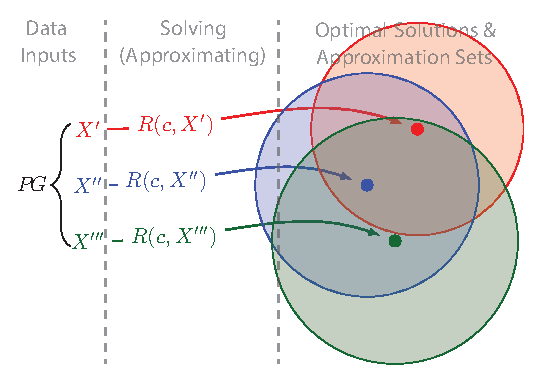
\includegraphics[width=\linewidth]{figures/ch_generic_approach/asc_coding_approximation_1}
            \caption{Large $\gamma$: approximation sets are in a great agreement, but non-informative at all.\\}
            \label{fig:asc_illustration-0}
        \end{subfigure}
        \hfill
        \begin{subfigure}[b]{.48\textwidth}
            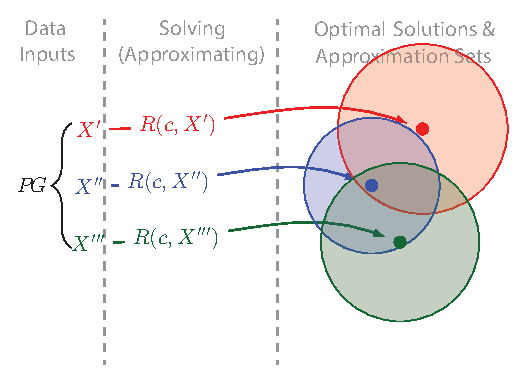
\includegraphics[width=\linewidth]{figures/ch_generic_approach/asc_coding_approximation_2}
            \caption{Decreasing $\gamma$: approximation sets get distinguished, and more information is extracted.}
            \label{fig:asc_illustration-1}
        \end{subfigure}
        \\[.5cm]
        % \begin{subfigure}[b]{.48\textwidth}
        %     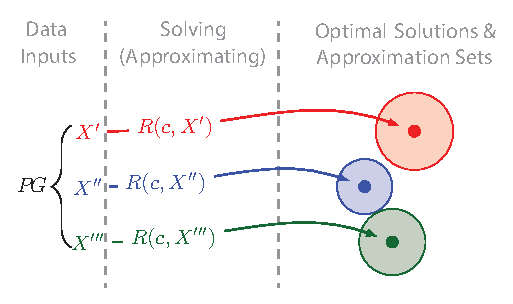
\includegraphics[width=\linewidth]{figures/ch_generic_approach/asc_coding_approximation_3}
        %     \caption{Further decreasing $\gamma$: approximation sets get distinguished, and more information is extracted.}
        %     \label{fig:asc_illustration-2}
        % \end{subfigure}
        % \hfill
        \begin{subfigure}[b]{.48\textwidth}
            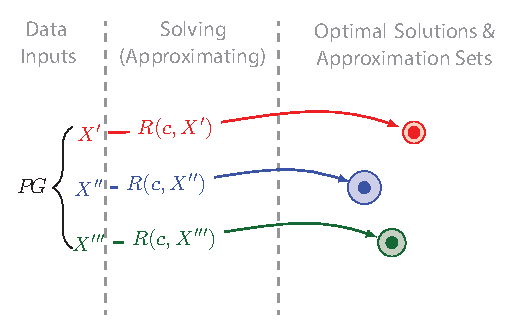
\includegraphics[width=\linewidth]{figures/ch_generic_approach/asc_coding_approximation_4}
            \caption{Small $\gamma$: almost all the information is extracted, but solutions are in poor agreement.}
            \label{fig:asc_illustration-3}
        \end{subfigure}
        \\[.5cm]
        \caption{Intuitive illustration of informativeness vs. stability.
          Approximation sets are parametrized by $\gamma$. The data inputs $X'$,
          $X''$ and $X'''$ come from the same generative source. Decreasing the
          parameter $\gamma$ leads to extracting more information from the given
          data, but at the same time making solutions less stable.}
        \label{fig:asc_illustration}
\end{figure}

Properties of the parameter $\gamma$ are crucial for understanding its role.
On one hand, it is obvious that infinite $\gamma$ yields the whole set of
feasible solutions:
\[
    \left.\mathcal{C}_{\gamma} \right|_{\gamma = \infty} (X) 
      \equiv \mathcal{C}.
\]
On the other hand, it holds
\[
    \left.\mathcal{C}_{\gamma} \right|_{\gamma = 0} (X) 
      \equiv \mathcal{C}^\bot(X) 
      \equiv \{c^\bot(X)\},
\]
i.e. zero $\gamma$ yields only optimal solutions. Selection of the parameter
$\gamma$ allows to trade-off stability of the solutions (extreme case: $\gamma =
\infty$) and the their informativeness (extreme case: $\gamma = 0$). This raises
a very important question: does there exist a way to choose this parameter?

\subsection{Communication and Learning Stability}
\label{sec:communication_learning_stability}

\begin{figure}[bh!]
  \centering
  \begin{subfigure}[b]{.48\textwidth}
      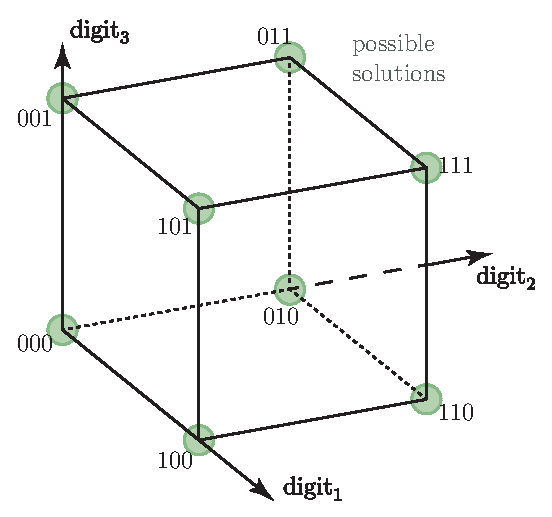
\includegraphics[width=\linewidth]{figures/ch_generic_approach/Boolean_Cube_8code}
      \caption{}
      \label{fig:boolen_cube_vectors_8}
  \end{subfigure}
  \hfill
  \begin{subfigure}[b]{.48\textwidth}
      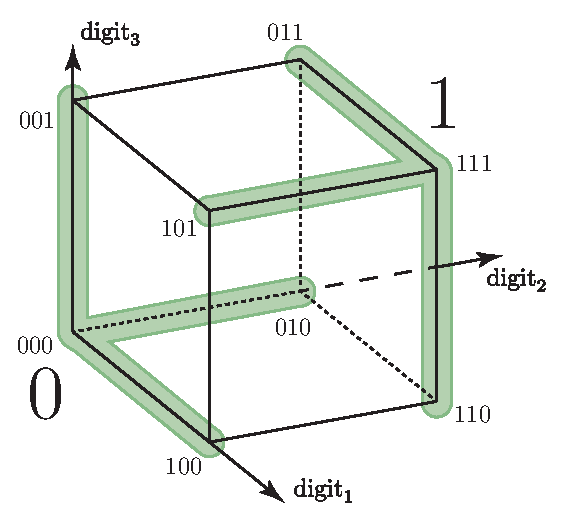
\includegraphics[width=\linewidth]{figures/ch_generic_approach/Boolean_Cube_2code}
      \caption{}
      \label{fig:boolen_cube_vectors_2}
  \end{subfigure}
  \\[.5cm]
  \caption{Placing codebook vectors of length $3$ on a Boolean cube. Case \textbf{(a)}
    is a ``mean'' option, when we use all the eight vertices as codebook vectors. 
    Case \textbf{(b)} is a ``lean'' option, when we use some of vertices as 
    neighborhoods to the two codebook vectors $000$ and $111$ denoted as big $0$ and big $1$.}
  \label{fig:boolen_cube_vectors}
\end{figure}

\begin{figure}[th!]
  \centering
  \begin{subfigure}[b]{.85\textwidth}
      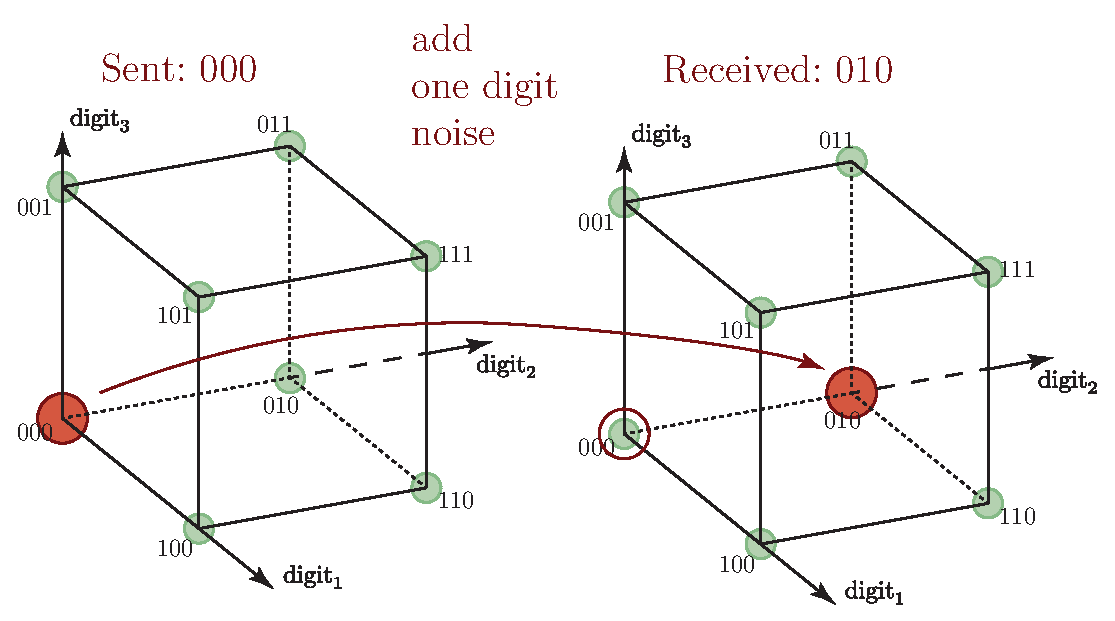
\includegraphics[width=\linewidth]{figures/ch_generic_approach/Boolean_Cube_8code_error}
      \caption{High rate ($R_{\text{code}}=1$), but no way to correct the error
      (red: sent and received codes).}
      \label{fig:boolen_cube_vectors_error_8}
  \end{subfigure}
  \\[.5cm]
  \begin{subfigure}[b]{.85\textwidth}
      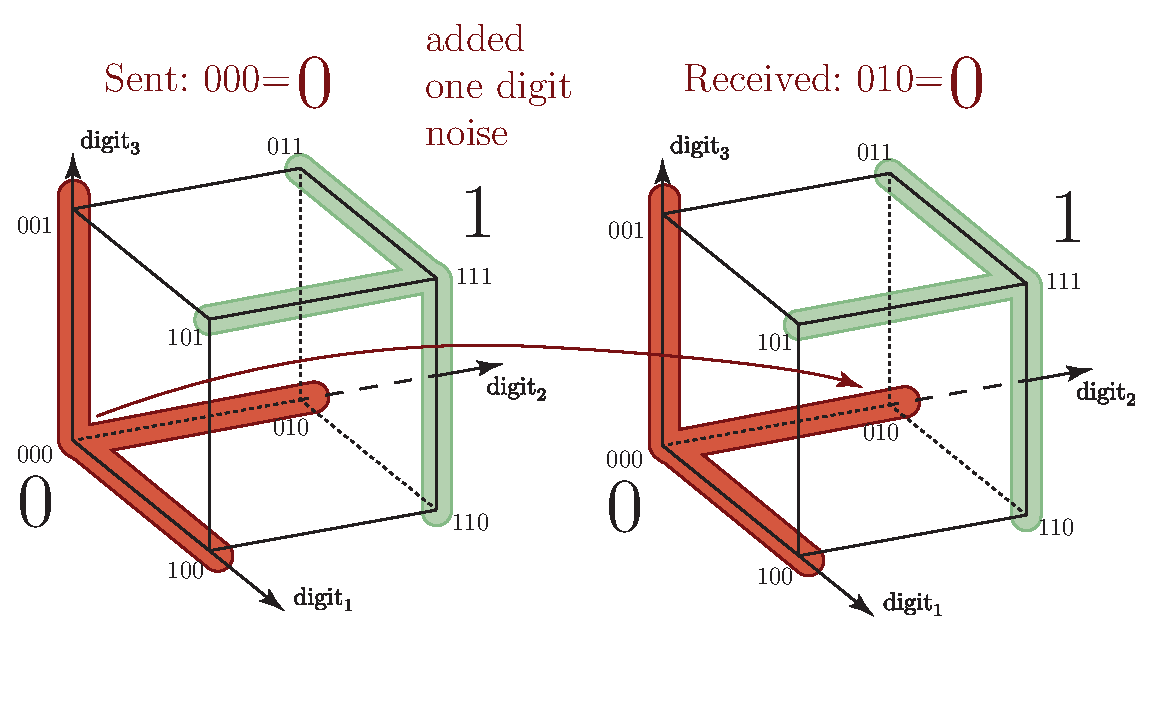
\includegraphics[width=\linewidth]{figures/ch_generic_approach/Boolean_Cube_2code_error}
      \caption{Lower rate ($R_{\text{code}} = 1/3$), correcting one digit error
      (red: sent and received codes).}
      \label{fig:boolen_cube_vectors_error_2}
  \end{subfigure}
  \\[.5cm]
  \caption{Dealing with one digit error. Case \textbf{(a)}
    is high rate option with eight codebook vectors, leading to a low
    error-correcting capacity (in fact, no error can be tolerated). Case
    \textbf{(b)} is lower rate option with two codebook vectors leading to a
    higher error-correcting capacity (one digit error can be tolerated, two
    digits not).}
  \label{fig:boolen_cube_vectors_error}
\end{figure}

In this section, we will be working under definitions of
Section~\ref{sec:background_coding}. The approximation set-based approach has clear
analogies in communication, featuring the idea of communication by means of data
and solutions. To illustrate this relation, we first will refer to information
theory and coding. As established by~\citet{shannon:1948, shannon:1963}, all the
rates up to channel capacity are achievable with vanishing error.

\index{Shannon's Channel Coding Theorem}
\newtheorem*{shannon_thm}{Shannon's Channel Coding Theorem}
\begin{shannon_thm}[e.g. Theorem 7.7.1, \citealp{Cover:2006}]
  For a discrete memoryless channel, all rates below capacity $C$ are
  achievable. Specifically, for every rate $R_{\text{code}} < C$, there exists a sequence of
  $(2^{nR_{\text{code}}}, n)$ codes with maximum probability of error $\lambda^{(n)} \to 0$.
  Conversely, any sequence of $(2^{nR_{\text{code}}}, n)$ codes with $\lambda^{(n)} \to 0$
  must have $R_{\text{code}} \le C$.
\end{shannon_thm}

This important theoretical statement has a non-constructive
proof resting on the idea of random coding with code length $n$ going to
infinity, and thus it does not provide a practical way of building such codes of
finite length. It turns out, that an attempt to design a finite-sized code faces
the trade-off between its error-correcting capability and its rate. An example
of this idea is the simplest Hamming code of length $3$ which we are going to
briefly illustrate due to its importance for the next steps.
\index{Trade-off!Error-correcting capability}
\index{Trade-off!Code rate}
\index{Hamming code}


Figures~\ref{fig:boolen_cube_vectors} and~\ref{fig:boolen_cube_vectors_error} to
some extent explain this trade-off in the simplest possible setting, thus
preparing the reader for introducing the communication channel by means of
datasets. Figure~\ref{fig:boolen_cube_vectors} shows that one can vary the
codebook vector set by, for instance, expanding ``neighborhoods'' of two
vertices $(000)$ and $(111)$ by including all the adjacent vectors, while
Figure~\ref{fig:boolen_cube_vectors_error} demonstrates that although the above
process reduces the code rate from $R_{\text{code}} = 1$ down to
$R_{\text{code}} = 1/3$, it increases its error-correcting capability so that
the code can now tolerate all the one-digit errors. One can also imagine an
extreme (not shown in figures) case of high two-digit noise: it is easy to see
that under this condition, a reliable, stable communication is only possible
with \textit{only one} codebook vector and the \textit{zero rate}
($R_{\text{code}} = 0$). In other words, the code gets less informative, but
more robust. 
\index{Code!Rate}
\index{Codebook!Vectors}

\begin{algorithm}[th!]
\caption{Establishing the Communication}\label{alg:communication_establishing}
\KwData{\\
  \quad instance of the dataset $X' \in \mathcal{X}$, \\ 
  \quad solution set $\mathcal{C} = \{c\}$, \\ 
  \quad cost function $R(c, X)$, \\ 
  \quad set of transformations $\mathbb{T} = \{\tau\}$, where $\tau \colon \mathcal{X} \to \mathcal{X}$\\ 
  \quad parameter $\gamma$}
\KwResult{established communication scheme}

{Sender and Receiver agree on $R(c, X)$\;}
{Sender and Receiver agree on $X'$\;}
{Sender and Receiver agree on $\mathbb{T}$\;}
{Sender and Receiver agree on $\gamma$\;}
\tcp{Then, a coverage by approximation sets is generated:}
\ForEach{$\tau \in \mathbb{T}$}{
  {both Sender and Receiver generate a transformed dataset $\tau \circ X'$\;}
  {both Sender and Receiver compute $\gamma$-approximation set 
    $\mathcal{C}_\gamma(\tau \circ X')$\;}
}
\end{algorithm}

As well as in the coding scenario described above, the learning process can be
viewed as a noisy communication, where the model is a \textit{decoder} which tries
to figure out the solution to \textit{true (useful) signal} contained in the
noisy data. Thus, the following rough analogies can be pointed out:
\begin{itemize}
  \item The role of codebook vectors is played by solutions $c$ to the optimization
    problem $R(c,X)$.
  \item The role of errors is played by the noise generating process $PG()$
    (see.~\eqref{eq:data_gen_model}), which injects uncertainty into data $X$.
  \item The role of ``neighborhoods'' of codebook vectors from
    Figures~\ref{fig:boolen_cube_vectors_2}
    and~\ref{fig:boolen_cube_vectors_error_2} is played by approximation
    sets.
\end{itemize}

We are now going, following~\cite{conf/isit/Buhmann10}, to introduce an
artificial communication scenario~(Algorithms~\ref{alg:communication_establishing},
\ref{alg:communication_transmission} and~\ref{alg:communication_decoding}).
We advise the reader to compare the textual explanation with the pictorial one 
in Figure.~\ref{fig:coding_scheme_cartoon}.
\index{Approximation Set Coding!Communication scenario}
\index{Communication scenario|see{Approximation Set Coding}}

\begin{algorithm}[bh!]
\caption{Encoding and Transmission}\label{alg:communication_transmission}
\KwData{\\
  \quad instance of the dataset $X' \in \mathcal{X}$, \\ 
  \quad instance $X'' \in \mathcal{X}$ not known to receiver, \\
  \quad solution set $\mathcal{C} = \{c\}$, \\ 
  \quad cost function $R(c, X)$, \\ 
  \quad set of transformations $\mathbb{T} = \{\tau\}$, where $\tau \colon \mathcal{X} \to \mathcal{X}$\\ 
  \quad parameter $\gamma$}
  
\KwResult{a received message}
{Sender picks a $\tau_{\text{send}} \in \mathbb{T}$ and sends it\;}
{Sender encodes it by generating 
  a transformed dataset $\tau_{\text{send}} \circ X'$ and sends it\;}
{Sender sends $\tau_{\text{send}} \circ X'$\;}
\tcp{Channel noise comes in the next line:}
{Channel introduces error by applying transformation $\tau_{\text{send}}$ to a $X''$\;}
{Receiver receives $\tau_{\text{send}} \circ X''$ without knowing either $\tau_{\text{send}}$ or $X''$\;}
\end{algorithm}

\paragraph{Encoding step (Algorithm~\ref{alg:communication_establishing}
\index{Approximation Set Coding!Encoding and transmission}
and~\ref{alg:communication_transmission};
Fig.~\ref{fig:coding_scheme_cartoon_1})} Very briefly, the Sender-Receiver
analogy consists in distinguishing individual solutions by means of the noisy
datasets: Sender sends a message (defined below) encoded by the first dataset,
and Receiver receives this message, but perturbed by means of the second
dataset. More precisely, assuming the generative process $PG$
(see~\eqref{eq:data_gen_model}), the transmitted ``messages'' are the
transformations $\tau \in \mathbb{T}$ of the datasets, so
\begin{equation}
  \tau \in \mathbb{T}, \quad \tau \colon \mathcal{X} \to \mathcal{X}.
\end{equation}
\nomenclature[D, 01a]{$\mathbb{T}$}{set of messages}%
\nomenclature[D, 01b]{$\tau \in \mathbb{T}$}{message}%
Now, both Sender and Receiver are agreeing on the dataset $X'$, which will
play the role of the encoding ``benchmark''. Sender then picks a
transformation $\tau_{\text{send}}$ and encodes the message by means of $X'$ via
applying one to the other:
\begin{equation}
  X_{\text{send}} \coloneqq \tau_{\text{send}} \circ X',
\end{equation}
\nomenclature[D, 01c]{$X', X''$}{two instances (ASC scenario)}%
\nomenclature[D, 01da]{$\tau_{\text{send}}$}{message sent}%
and sends it out. Remember that Receiver does not know $\tau_{\text{send}}$, but knows
``codebook approximation sets'' $\{\tau \circ X'\}_{\tau \in \mathbb{T}}$.

\paragraph{Hypothetic noise-free transmission}
If there were no noise, Receiver, having obtained $X_\text{received} =
X_{\text{send}}$, and knowing both $\mathbb{T}$ and $X'$, could just recover the
$\tau_{\text{send}}$ by enumerating:
\begin{equation}
\label{eq:acs_brute_force_decoding}
  \hat \tau \coloneqq \arg \max_{\tau \in \mathbb{T}} \Ind\{X_{\text{received}} = 
    \tau \circ X' \}.
\end{equation}
\nomenclature[D, 01db]{$\hat \tau$}{message decoded}%

\paragraph{Actual noisy transmission (Algorithm~\ref{alg:communication_transmission}; 
Fig.~\ref{fig:coding_scheme_cartoon_2})} 
However, the noise is injected by replacing 
$X'$ by $X''$, which is a noisy version of the initial dataset:
\begin{equation}
  X_{\text{received}} \coloneqq \tau_{\text{send}} \circ X'',
\end{equation}
which makes it impossible for Receiver to perfectly match obtained message to
any of the ``benchmarked ones'' like in Eq.~\eqref{eq:acs_brute_force_decoding}.

\parsec
\myremark It it important to realize, that there are two manifestations of noise
in this scenario. One is the original source of noise generated by $PG(\cdot)$ and resulting
in replacing $X'$ by $X''$. The other is the transmission error caused by 
difference between the sent and received messages.

\paragraph{Decoding (Algorithm~\ref{alg:communication_decoding}; Fig.~\ref{fig:coding_scheme_cartoon_3} and
\ref{fig:coding_scheme_cartoon_4})} 
Just the same
as the Hamming channel performs decoding the received vector by finding
the closest codebook vector, our Receiver tries to find the closest codebook 
dataset out of all the possible datasets $\{\tau \circ X'\}_{\tau \in \mathbb{T}}$.
Closeness is measured as the size of the intersection of their approximation sets:
\begin{equation}
  \hat \tau = \arg \max_{\tau \in \mathbb{T}} \,\,
  \bigl| 
     \mathcal{C}_\gamma(\tau \circ X') \cap \mathcal{C}_\gamma(\tau_{\text{send}} \circ X'')
  \bigr|,
\end{equation}
thus, approximation sets play the role of parity check regions here.
\index{Parity check}

\begin{algorithm}[t]
\caption{Decoding}\label{alg:communication_decoding}
\KwData{\\
  \quad instance of the dataset $X' \in \mathcal{X}$, \\ 
  \quad instance $X'' \in \mathcal{X}$ not known to receiver, \\
  \quad solution set $\mathcal{C} = \{c\}$, \\ 
  \quad cost function $R(c, X)$, \\ 
  \quad set of transformations $\mathbb{T} = \{\tau\}$, where $\tau \colon \mathcal{X} \to \mathcal{X}$\\ 
  \quad parameter $\gamma$}
\KwResult{Transformation $\hat \tau$ which is estimate for $\tau_{\text{send}}$}
{Receiver computes a $\gamma$-approximation set of the received dataset: 
$\mathcal{C}_\gamma(\tau_{\text{send}} \circ X'')$\;}
{Receiver maximizes its overlap with known $\gamma$-approximation sets: 
\begin{equation}\label{eq:asc_decoding_intersection}
  \hat \tau = \arg \max_{\tau \in \mathbb{T}} \,\,
  \bigl| 
     \mathcal{C}_\gamma(\tau \circ X') \cap \mathcal{C}_\gamma(\tau_{\text{send}} \circ X'')
  \bigr|
\end{equation}}
\index{Approximation Set Coding!Decoding}
\end{algorithm}

\index{Hamming code!Decoding}
\index{Hamming distance}
It is crucially important to realize that this decoding rule is very similar to
that of the Hamming code (and thus very natural), because in the Hamming coding,
the closeness is measured by \textit{minimizing} the Hamming distance between
the received vector and the codebook vectors, which is the same as
\textit{maximizing} the intersection between them:
\begin{align}
  \hat{\mathbf{x}} &= 
    \arg \min_{\mathbf{x} \in \mathbb{B}^3} \;
      \|\textbf{x}_\text{received} \oplus \textbf{x} \| \notag \\ 
    &= \arg \min_{\mathbf{x} \in \mathbb{B}^3} \; \bigl( n - 
        \|\textbf{x}_\text{received} \cap \textbf{x}\| \bigr) \notag \\
    &=  \arg \max_{\mathbf{x} \in \mathbb{B}^3} \;
         \|\textbf{x}_\text{received} \cap \textbf{x}\|.
\end{align}
\nomenclature[A, 00]{$\mathbb{B}^3$}{Boolean cube}%
\nomenclature[A, 00a]{$\oplus$}{sum modulo $2$}%

\paragraph{Decoding error and its probability}

When $\hat \tau \ne \tau_\text{send}$, we say that a decoding error occurs.
Obviously, the noise in our channel
(Algorithm~\ref{alg:communication_transmission}), acting via $PG(\cdot | X^0)$,
is the reason for that. Transferring robust optimization problem into a robust
decoding problem, we now will answer, following~\citet{conf/isit/Buhmann10}, a
natural question: how can we bound this probability?

We are interested in bounding the probability
\begin{equation}
  \Prob(\hat \tau \ne \tau_\text{send} | \tau_\text{send}).
\end{equation}

\begin{figure}[th!]
  \centering
  \begin{subfigure}[b]{.48\textwidth}
      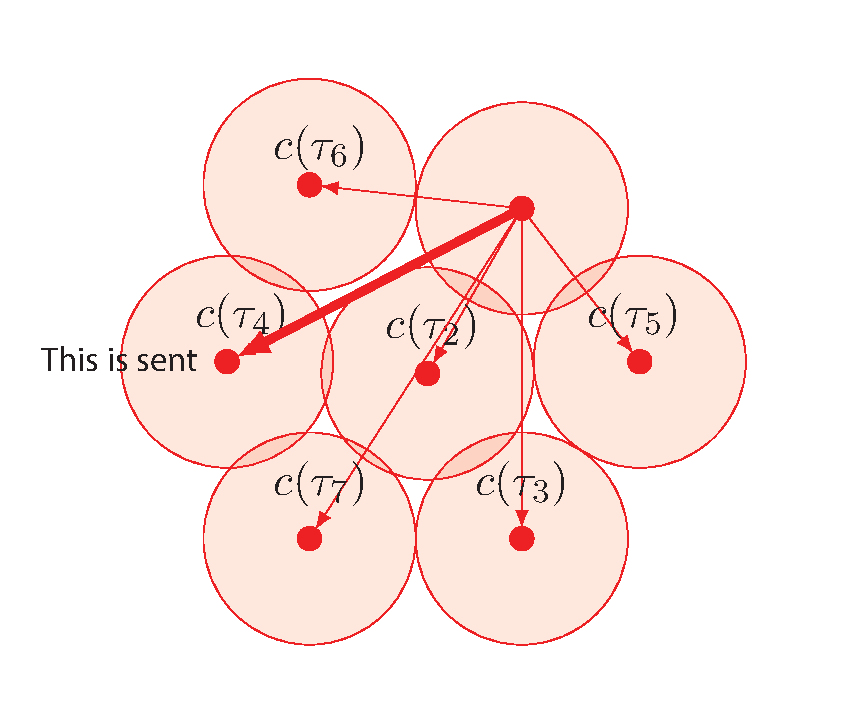
\includegraphics[width=\linewidth]{figures/ch_generic_approach/coding_scheme_1}
      \caption{}
      \label{fig:coding_scheme_cartoon_1}
  \end{subfigure}
  \hfill
  \begin{subfigure}[b]{.48\textwidth}
      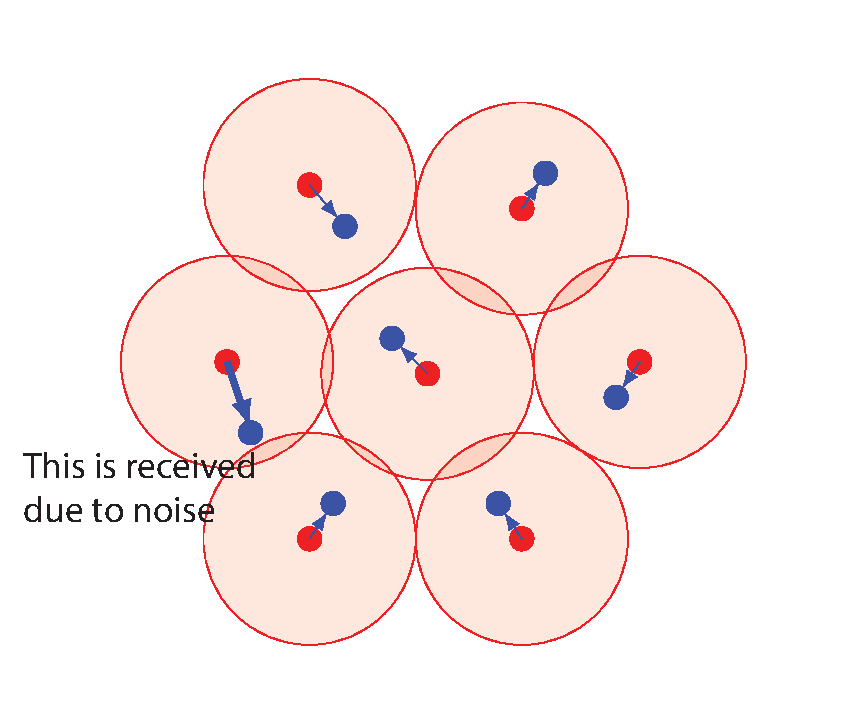
\includegraphics[width=\linewidth]{figures/ch_generic_approach/coding_scheme_2}
      \caption{}
      \label{fig:coding_scheme_cartoon_2}
  \end{subfigure}
  \\[.5cm]
  \begin{subfigure}[b]{.48\textwidth}
      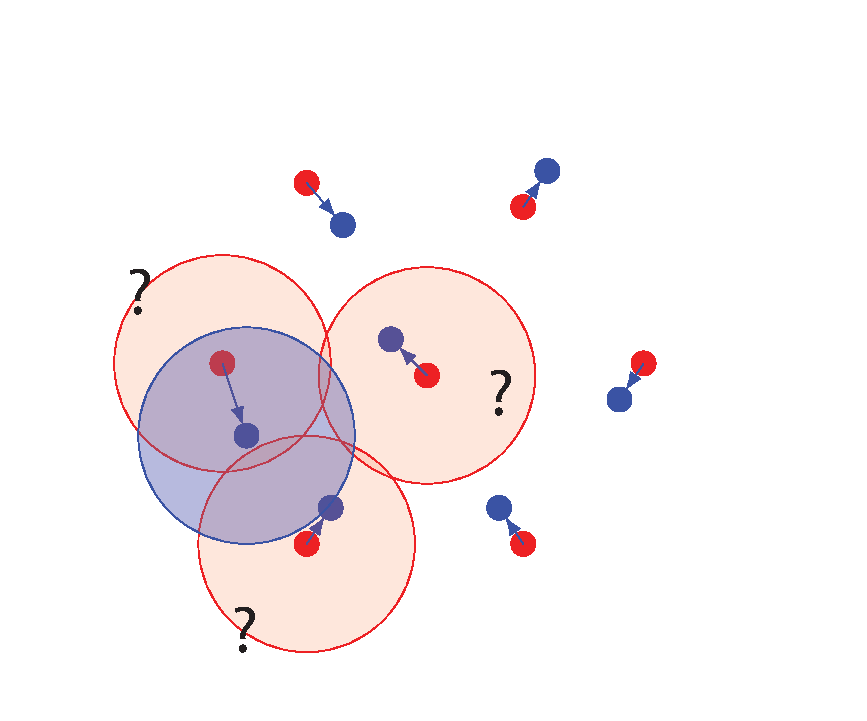
\includegraphics[width=\linewidth]{figures/ch_generic_approach/coding_scheme_3}
      \caption{}
      \label{fig:coding_scheme_cartoon_3}
  \end{subfigure}
  \hfill
  \begin{subfigure}[b]{.48\textwidth}
      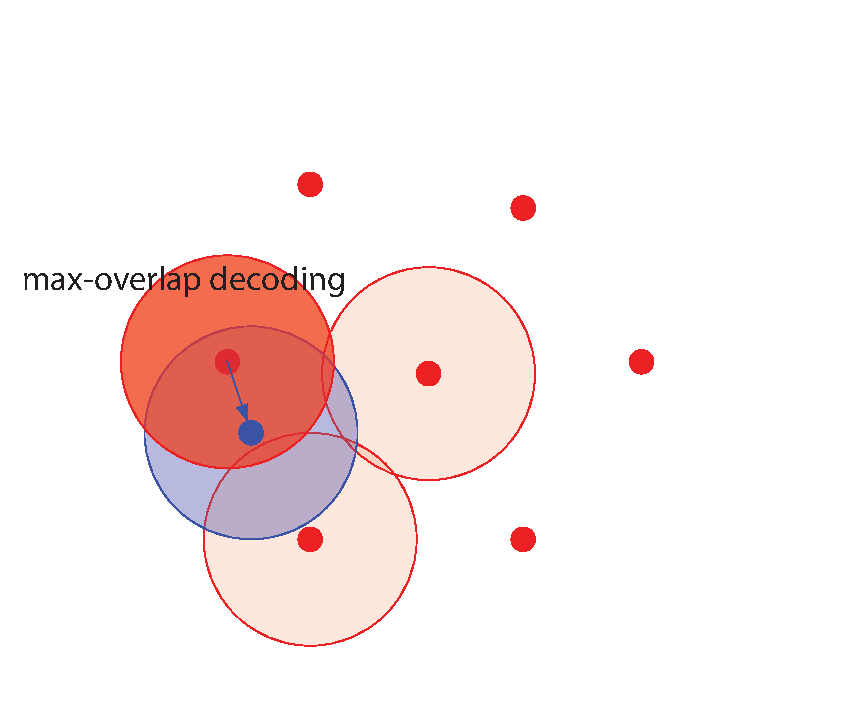
\includegraphics[width=\linewidth]{figures/ch_generic_approach/coding_scheme_4}
      \caption{}
      \label{fig:coding_scheme_cartoon_4}
  \end{subfigure}
  \\[.5cm]
  \caption{Process of correct decoding by approximation sets in the solution
    space: \textbf{(a)} $X'$ is set and sender sends $\tau_4$; \textbf{(b)} due
    to noise which replaces $X'$ by $X''$, all the minimizers move around (red
    to blue) in the solution space; \textbf{(c)} the received solution is
    surrounded by its approximation set (blue) and overlaps are considered;
    \textbf{(d)} decoded solution (dark red) happens to be $\tau_4$ which was initially
    sent (correct decoding).}
  \label{fig:coding_scheme_cartoon}
\end{figure}

Before we proceed, we will denote the intersection in~\eqref{eq:asc_decoding_intersection}
as follows:
\begin{equation}
  \Delta \mathcal{C}_\gamma^\tau 
    \coloneqq \mathcal{C}_\gamma(\tau \circ X') 
      \cap \mathcal{C}_\gamma(\tau_{\text{send}} \circ X'').
\end{equation}
Due to the union bound, it holds that \index{Union bound}
\begin{equation}
  \Prob(\hat \tau \ne \tau_\text{send} | \tau_\text{send}) 
    \le \sum_{\tau \in \mathbb{T}} \Prob 
      \bigl(
        |\Delta \mathcal{C}_\gamma^\tau| \ge |\Delta \mathcal{C}_\gamma^{\tau_\text{send}}| \bigm| \tau_\text{send}
      \bigr),
\end{equation}
i.e. for decoding error to occur, one has to encounter an approximation set
which is yielded by a wrong transformation, but happens to be closer to the
received approximation set (this is illustrated in
Figure~\ref{fig:coding_scheme_cartoon_7}). The last bound can be rewritten via
the indicator function:
\begin{equation}
  \Prob(\hat \tau \ne \tau_\text{send} | \tau_\text{send}) 
    \le \sum_{\tau \in \mathbb{T}} \Expct_{PG}
      \bigl[
        \Ind\{|\Delta \mathcal{C}_\gamma^\tau| \ge |\Delta \mathcal{C}_\gamma^{\tau_\text{send}}|\} \bigm| \tau_\text{send}
      \bigr],
\end{equation}
where the expectation is taken w.r.t. the problem generation process $X', X''
\sim PG(\cdot | X^0)$. We further utilize the monotonicity of $\log$ function:
\begin{equation}
  \Ind\{|\Delta \mathcal{C}_\gamma^\tau| \ge |\Delta \mathcal{C}_\gamma^{\tau_\text{send}}|\} 
  = \Ind\{\log |\Delta \mathcal{C}_\gamma^\tau| \ge \log |\Delta \mathcal{C}_\gamma^{\tau_\text{send}}|\} 
\end{equation}
and the fact that $\Ind\{x \ge 0\} \le \exp(x)$ to come to the following:
\begin{equation}
  \Expct_{PG}
      \Bigl(
        \Ind\{|\Delta \mathcal{C}_\gamma^\tau| \ge |\Delta \mathcal{C}_\gamma^{\tau_\text{send}}|\} \Bigm| \tau_\text{send}
      \Bigr)
      \le
      \frac{|\mathcal{C}_\gamma(X')| \;  |\mathcal{C}_\gamma(X'')|}%
      {|\mathbb{T}| \; |\Delta \mathcal{C}_\gamma^{\tau_\text{send}}|},
\end{equation}
where the product in the nominator comes from the fact that, under our
generation process, the data instances $X'$ and $X''$ are independent given
$X^0$, see~\eqref{eq:pg_independence}.

In the spirit of~\citet{shannon:1948}, we use the random coding argument here: 
all the $\tau$ are identically distributed and independent, hence the above can
be rewritten:
\begin{equation}
  \Prob(\hat \tau \ne \tau_\text{send} | \tau_\text{send}) \le (|\mathbb{T}| - 1)
    \exp(- I_\gamma(\tau_\text{send}, \hat \tau)),
\end{equation}
where 
\begin{equation}
  I_\gamma(\tau_\text{send}, \hat \tau) \coloneqq  \Expct \log 
  \Bigl(
    \frac{|\mathbb{T}| \; |\Delta \mathcal{C}_\gamma^{\tau_\text{send}}|}%
      {|\mathcal{C}_\gamma(X')| \;  |\mathcal{C}_\gamma(X'')|}
  \Bigr).
\end{equation}

\paragraph{Optimizing approximation parameter $\boldsymbol\gamma$}
At this point, we can determine the optimal $\gamma^*$ as follows: the optimal
approximation threshold is chosen as
\begin{equation}\label{eq:asc_best_gamma}
  \gamma^* = \arg \max_{\gamma \ge 0} I_\gamma(\tau_\text{send}, \hat \tau).
\end{equation}
\nomenclature[D, 01]{$\gamma^*$}{optimal $\gamma$}%

\begin{figure}[th!]
  \centering
  \begin{subfigure}[b]{.48\textwidth}
      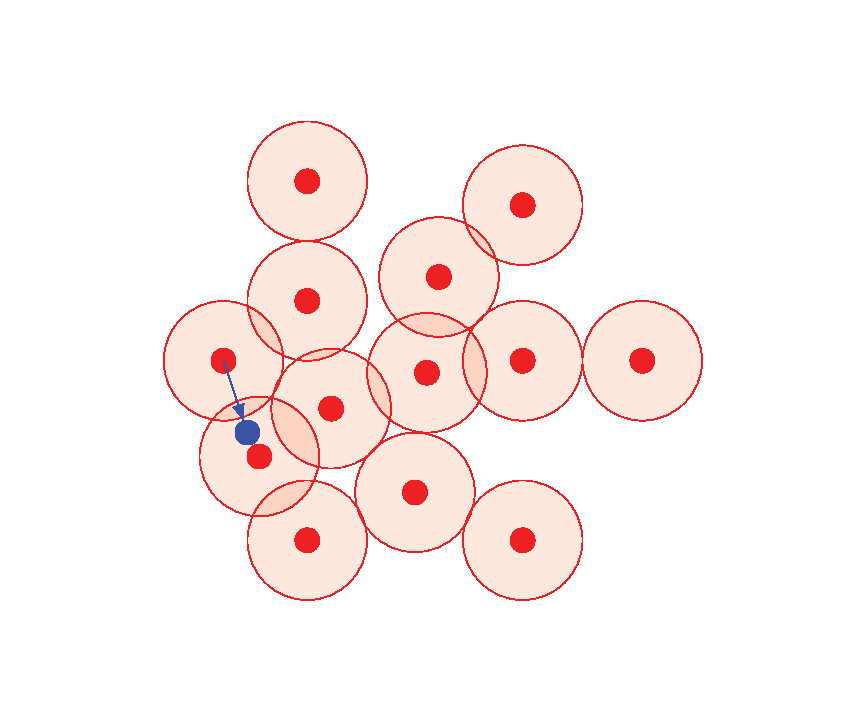
\includegraphics[width=\linewidth]{figures/ch_generic_approach/coding_scheme_5}
      \caption{}
      \label{fig:coding_scheme_cartoon_5}
  \end{subfigure}
  \\[.5cm]
  \begin{subfigure}[b]{.48\textwidth}
      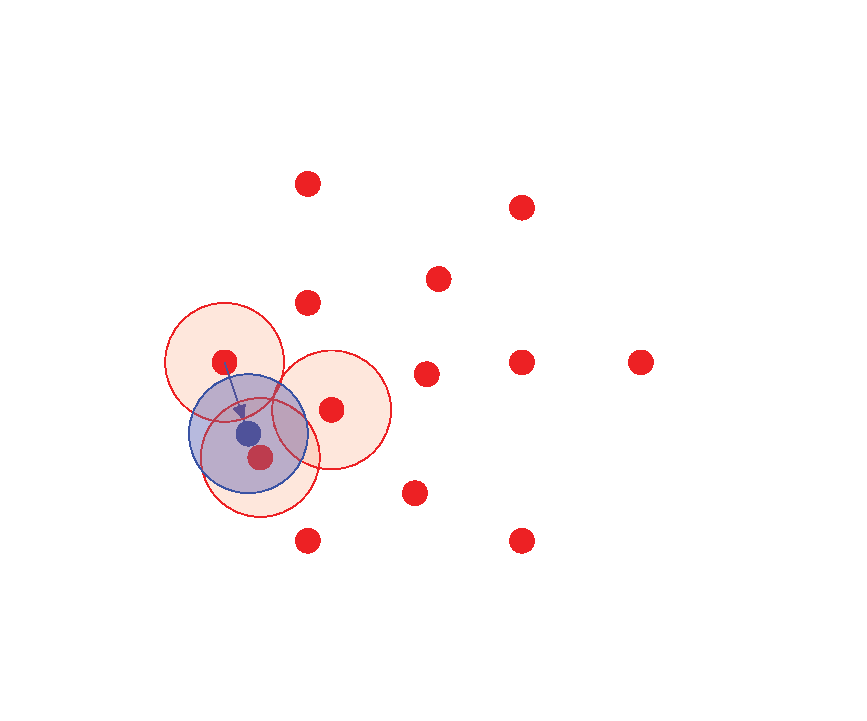
\includegraphics[width=\linewidth]{figures/ch_generic_approach/coding_scheme_6}
      \caption{}
      \label{fig:coding_scheme_cartoon_6}
  \end{subfigure}
  \hfill
  \begin{subfigure}[b]{.48\textwidth}
      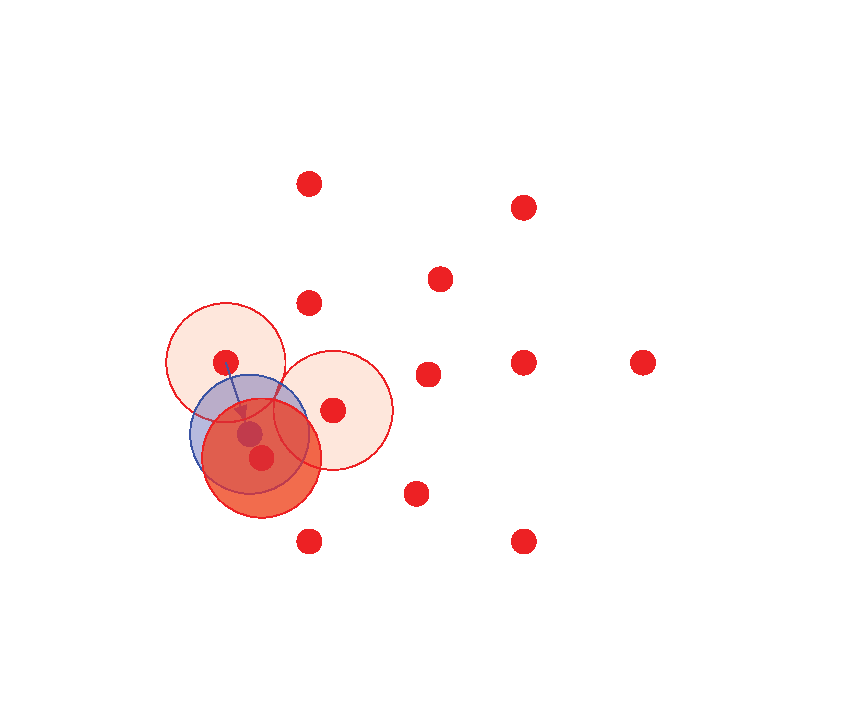
\includegraphics[width=\linewidth]{figures/ch_generic_approach/coding_scheme_7}
      \caption{}
      \label{fig:coding_scheme_cartoon_7}
  \end{subfigure}
  \\[.5cm]
  \caption{Decreased $\gamma$ and increased code rate leads to incorrect
    decoding: \textbf{(a)} same setting (i.e. same noise) as in
    Figure~\ref{fig:coding_scheme_cartoon}, but added more codebook
    vectors; \textbf{(b)} due to noise which replaces $X'$ by $X''$, all the
    minimizers move around (red to blue) in the solution space, \textbf{(c)}
    decoded solution (dark red) happens to be wrong (incorrect decoding).}
  \label{fig:coding_scheme_cartoon_incorrect}
\end{figure}

In practical applications and in the spirit of the Shannon's random coding
argument, it is often assumed that that $\tau_\text{send} = \mathrm{Id}$, i.e.
one computes
\begin{equation}
  I_\gamma(\tau_\text{send}, \hat \tau) \coloneqq  \Expct \log 
  \Bigl(
    \frac{|\mathbb{T}| \; |\Delta \mathcal{C}_\gamma(X', X'')|}%
      {|\mathcal{C}_\gamma(X')| \; |\mathcal{C}_\gamma(X'')|}
  \Bigr),
\end{equation}
where
\begin{equation}
  \Delta \mathcal{C}_\gamma \coloneqq \mathcal{C}_\gamma(X') 
      \cap \mathcal{C}_\gamma(X'').
\end{equation}
\nomenclature[D, 01]{$\Delta \mathcal{C}_\gamma$}{intersection of approximation sets}%
In practice, one often replaces $|\mathbb{T}|$ with the cardinality of the full
solution set~\citep{morteza12}, reflecting a specific choice of possible
transformations\footnote{Since the proof of error probability rests on the
argument of random coding and the codebook messages are chosen randomly, all
the considerations remain valid.}:
\begin{equation}\label{eq:asc_mutual_information_formula}
  I_\gamma(\tau_\text{send}, \hat \tau) \coloneqq  \Expct \log 
  \Bigl(
    \frac{|\C| \; |\Delta \mathcal{C}_\gamma(X', X'')|}%
      {|\mathcal{C}_\gamma(X')| \; |\mathcal{C}_\gamma(X'')|}
  \Bigr),
\end{equation}
\nomenclature[D, 02a]{$I_\gamma$}{ASC $\gamma$-score}%
\begin{definition}
\label{def:asc_score}
  We will call the above quantity ASC $\gamma$-score. We will call its maximum
  simply ASC score or Approximation Capacity (AC):
  \begin{equation}
    C \coloneqq \max_\gamma I_\gamma.
  \end{equation}
  \nomenclature[D, 02ba]{$C$}{approximation capacity}%
  \index{ASC score}
  \index{Approximation capacity}
\end{definition}

\myremark It is interesting to note that the semantics of $I_\gamma(\tau_\text{send}, \hat
\tau)$ is surprisingly similar to that of mutual information
(Definition~\ref{def:inf_theory_mutual_information}). First, both are related to
the maximum rate of certain channel. Second,  both can be decomposed in quite a
similar way: recall from~\eqref{eq:background_mi_decomposition} that, for random
variables $X$ and $Y$,
\begin{equation*}
  \MI(X, Y) = H(X) + H(Y) - H(X, Y).
\end{equation*}
In a same way one may observe, that~\eqref{eq:asc_mutual_information_formula}
can be very easily decomposed into three logarithms:
\begin{align}
  I_\gamma(\tau_\text{send}, \hat \tau) =  \overbrace{- \Expct \log 
  \Bigl(
    \frac{|\mathcal{C}_\gamma(X')|}{ |\C| }
  \Bigr)}^{\text{single entropy}}
  %
  &\overbrace{- \Expct \log 
  \Bigl(
    \frac{|\mathcal{C}_\gamma(X'')|}{|\C|}
  \Bigr)}^{\text{single entropy}} \notag \\
  %
  &\underbrace{+\Expct \log 
  \Bigl(
    \frac{|\Delta \mathcal{C}_\gamma(X', X'')|}{ |\C| }
  \Bigr)}_{\text{joint entropy}},
\end{align}
where first two terms can be contemplated as single entropies of uniform
distributions over approximation sets, and the third term corresponds to
the joint entropy.

\myremark In practical applications, when there are only two data points $X'$, $X''$ and
no information about $PG(\cdot)$ is available, one can use an empirical version
of~\eqref{eq:asc_mutual_information_formula}
\begin{equation}\label{eq:asc_mutual_information_formula_wo_expct}
\hat I_\gamma(X', X'') \coloneqq  \log 
  \Bigl(
    \frac{|\C| \; |\Delta \mathcal{C}_\gamma(X', X'')|}%
      {|\mathcal{C}_\gamma(X')| \; |\mathcal{C}_\gamma(X'')|}
  \Bigr),
\end{equation}
\nomenclature[D, 02b]{$\hat I_\gamma$}{empirical ASC $\gamma$-score}%
as an estimator without the expectation sign. More on that will be given in
Chapter~\ref{ch:mst} when describing the application.

\section{Another View: Similarity Approach}
\label{sec:similarity_approach_intro}

In this section, we briefly visit, with sufficient adaptation of
notation\footnote{The two interpretations of the same idea have been
developed in parallel, hence there are two consistent systems of notation.},
another view on finding a robust approximation, which is called
\textit{similarity approach} and was introduced and developed, e.g.,
in~\citep{Sramek:PhD,Proeger:PhD,jcss:2017}. Yielding the same quantity as
in~\eqref{eq:asc_best_gamma}, this approach arose from a specific interpretation
of the ASC~\citep{conf/isit/Buhmann10}.
\index{Similarity approach}

For the sake of itegration into the thesis, in this section we use additive
approximation set notation (i.e. the same as everywhere in this thesis),
while~\citet{Sramek:PhD} used a multiplicative one\footnote{For the definiton of
multiplicative approximation sets, refer to e.g.~\citep{Sramek:PhD} or
\citep{jcss:2017}.}. Assume there are two \textit{data instances} $X'$ and
$X''$, coming from the same source~$PG(\cdot | X^0)$,
see~\eqref{eq:data_gen_model}. \citet{Sramek:PhD} identifies two cases:

\begin{itemize}
  \item If the generation process $PG$ is very noisy, resulting in two
  non-similar instances $X'$ and $X''$ it is obvious that the intersection of
  two approximation sets ${\mathcal{C}_\gamma}(X')\cap
  {\mathcal{C}_\gamma}(X'')$ will contain some solutions when $\gamma$ is large
  enough. \citet{Sramek:PhD} calls such solutions \emph{expected
  due to $\gamma$}. At this point, the reader can start building analogies to
  the above by revisiting Figure~\ref{fig:asc_illustration-0}, where large
  approximation sets yield a lot of solutions in the intersection.

  \item On the other hand, if the two instances $X'$ and $X''$ are more similar,
  which is the case for a low-noise $PG$, the intersection
  ${\mathcal{C}_\gamma}(X')\cap {\mathcal{C}_\gamma}(X'')$, taken at the same
  $\gamma$ value, will contain, in addition to the above-mentioned (expected due
  to $\gamma$) ones, some solutions due to the similarity of the instances.
  \citet{Sramek:PhD} calls them \emph{unexpected}. In terms coined later~\citep{jcss:2017} 
  it is called \emph{expected due to similarity}.
  \index{Solutions!Expected due to similarity}
\end{itemize}

The point of introducing such cases consists in the following: these latter
solutions,~--- i.e. the ones expected due to similarity~--- are likely to be
good choices for possible test instance $X'''$ that comes from the same source.

The goal is thus shifted to finding the $\gamma$ that maximizes the ratio of the
number of solutions that are expected due to similarity over the size of the
intersection (compare to the ASC approach~\eqref{eq:asc_best_gamma}; the
comparison will be summarized in conclusion,
Section~\ref{sec:gen_appch_conclusion}). To fulfill the task, several
definitions are required. Figure~\ref{fig:intersection_types} illustrates these
definitions.

\begin{definition}[Feasible approximation set] \label{def:feasible_as}
  A set of solutions $F\subseteq\mathcal{C}$ is called a
  \emph{feasible approximation set} if there exists some instance $\tilde X$ and
  some number $\tilde \gamma$ such that $F$ is the $\tilde \gamma$-approximation
  set of $\tilde X$.
\end{definition}

\begin{definition}[Expected intersection sizes due to $\gamma$] \label{def:intersection_due_to_gamma}
  Given $\gamma$ and the sizes $|{\mathcal{C}_\gamma}(X')| =: k(\gamma)$ and
  $|{\mathcal{C}_\gamma}(X'')| =: l(\gamma)$, let
  $es(\gamma,k(\gamma),l(\gamma))$ denote the expected size of the intersection
  of two feasible approximation sets $A$ and $B$ of sizes $k(\gamma)$ and
  $l(\gamma)$, respectively.
  \nomenclature[D, 03a]{$es(\gamma,k(\gamma),l(\gamma))$}{expected intersection\nomnorefeqpage\hfill Def.~\ref{def:intersection_due_to_gamma}}%
\end{definition}
  
\begin{definition}[Expected intersection due to similarity] \label{def:intersection_due_to_sim}
  Given $\gamma$ and the sizes $|{\mathcal{C}_\gamma}(X')| =: k(\gamma)$ and
  $|{\mathcal{C}_\gamma}(X'')| =: l(\gamma)$, if the intersection of
  ${\mathcal{C}_\gamma}(X')$ and ${\mathcal{C}_\gamma}(X'')$ is larger than the
  expected size $es(\gamma,k(\gamma),l(\gamma))$, then it contains some
  solutions that are expected due to similarity, and we will denote them
  $sim(\gamma)$.
  \nomenclature[D, 03b]{$sim(\gamma)$}{size expected due to $\gamma$\nomnorefeqpage\hfill Def.~\ref{def:intersection_due_to_sim}}%
\end{definition}
%
%
\begin{figure}[t!]
  \centering
  \begin{subfigure}[b]{.55\textwidth}
      \label{fig:approx_sets--example--1} 
      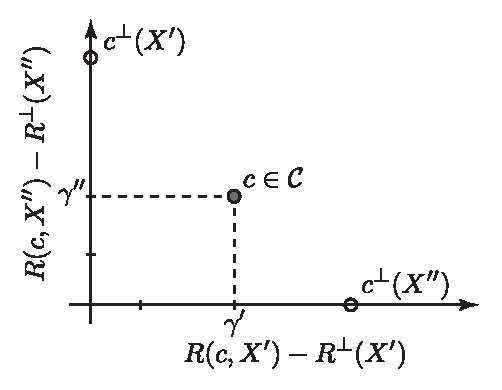
\includegraphics[width=\linewidth]{figures/ch_generic_approach/approx_sets--schematic--1}
      \caption{Placing a solution $c \in \C$}
  \end{subfigure}
  \\[.5cm]
  \begin{subfigure}[b]{.55\textwidth}
      \label{fig:approx_sets--example--3}
      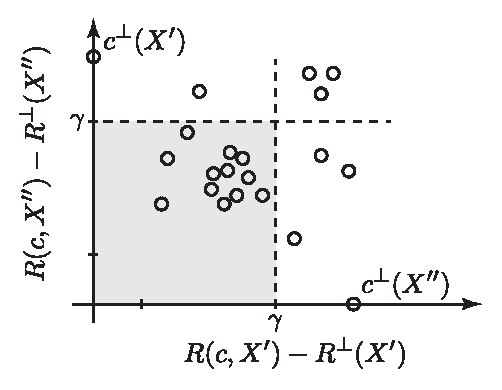
\includegraphics[width=\linewidth]{figures/ch_generic_approach/approx_sets--schematic--3}
      \caption{Intersection $\mathcal{C}_{\gamma}(X')\cap \mathcal{C}_{\gamma}(X'')$}
  \end{subfigure}
  \\[.5cm]
  \caption{
    Approximation sets for the instances $X'$ and $X''$. By $c^\bot(X)$ we
    denote the solution whose cost is minimum in $X$. \textbf{(a)}: We
    place each solution $c \in \mathcal{C}$ at position
    $(\gamma',\gamma'')$, where $\gamma'=R(c, X') - R^\bot(X')$ and
    $\gamma''=R(c, X'') - R^\bot(X'')$. \textbf{(b)}: Example of
    intersection of approximation sets $\mathcal{C}_{\gamma}(X')\cap
    \mathcal{C}_{\gamma}(X'')$ (this view on approximation sets was 
    originally suggested by Tobias Pröger~\citep[cf.][]{jcss:2017}, figure labels
    adapted for additive notation).}
  \label{fig:approx_sets--schematic}
\end{figure}
%
Thus we have 
\begin{equation}
  |{\mathcal{C}_\gamma}(X') \cap {\mathcal{C}_\gamma}(X'')|=sim(\gamma)+
    es(\gamma,k(\gamma),l(\gamma)),
\end{equation}
and, to maximize the probability that the uniformly randomly
chosen solution from the intersection is stable, we want to find the value $\gamma$ that maximizes
$\frac{sim(\gamma)}{sim(\gamma)+es(\gamma,k(\gamma),l(\gamma))}$. The following about 
maximization objectives holds:
\begin{align}
  \arg \max_{\gamma>0} &\;\; \frac{sim(\gamma)}{sim(\gamma)+es(\gamma,k(\gamma),l(\gamma))}  \notag \\
    &\qquad= \arg \max_{\gamma > 0} \; \Bigl(
        1 - \frac{es(\gamma,k(\gamma),l(\gamma))}{sim(\gamma)+es(\gamma,k(\gamma),l(\gamma))}
      \Bigr) \notag \\
    &\qquad= \arg \min_{\gamma > 0} \;\; \frac{es(\gamma,k(\gamma),l(\gamma))}{sim(\gamma)+es(\gamma,k(\gamma),l(\gamma))}
      \notag \\
    &\qquad= \arg \max_{\gamma > 0} \;\; \frac{sim(\gamma)+es(\gamma,k(\gamma),l(\gamma))}{es(\gamma,k(\gamma),l(\gamma))},
\end{align}
hence we can reformulate (for the sake of clarity) the objective of the similarity-based
approach as maximizing the value
\begin{align}
  \label{eq:similarity}
  S_\gamma(X',X'')
    \coloneqq \frac{|{\mathcal{C}_\gamma}(X') \cap {\mathcal{C}_\gamma}(X'')|}{es(\gamma,k(\gamma),l(\gamma))}
    = \frac{sim(\gamma)+es(\gamma,k(\gamma),l(\gamma))}{es(\gamma,k(\gamma),l(\gamma))}.
\end{align}


\begin{figure}[t!]
  \centering
  \begin{subfigure}[b]{.49\textwidth}
      \label{fig:intersection_due_to_gamma} 
      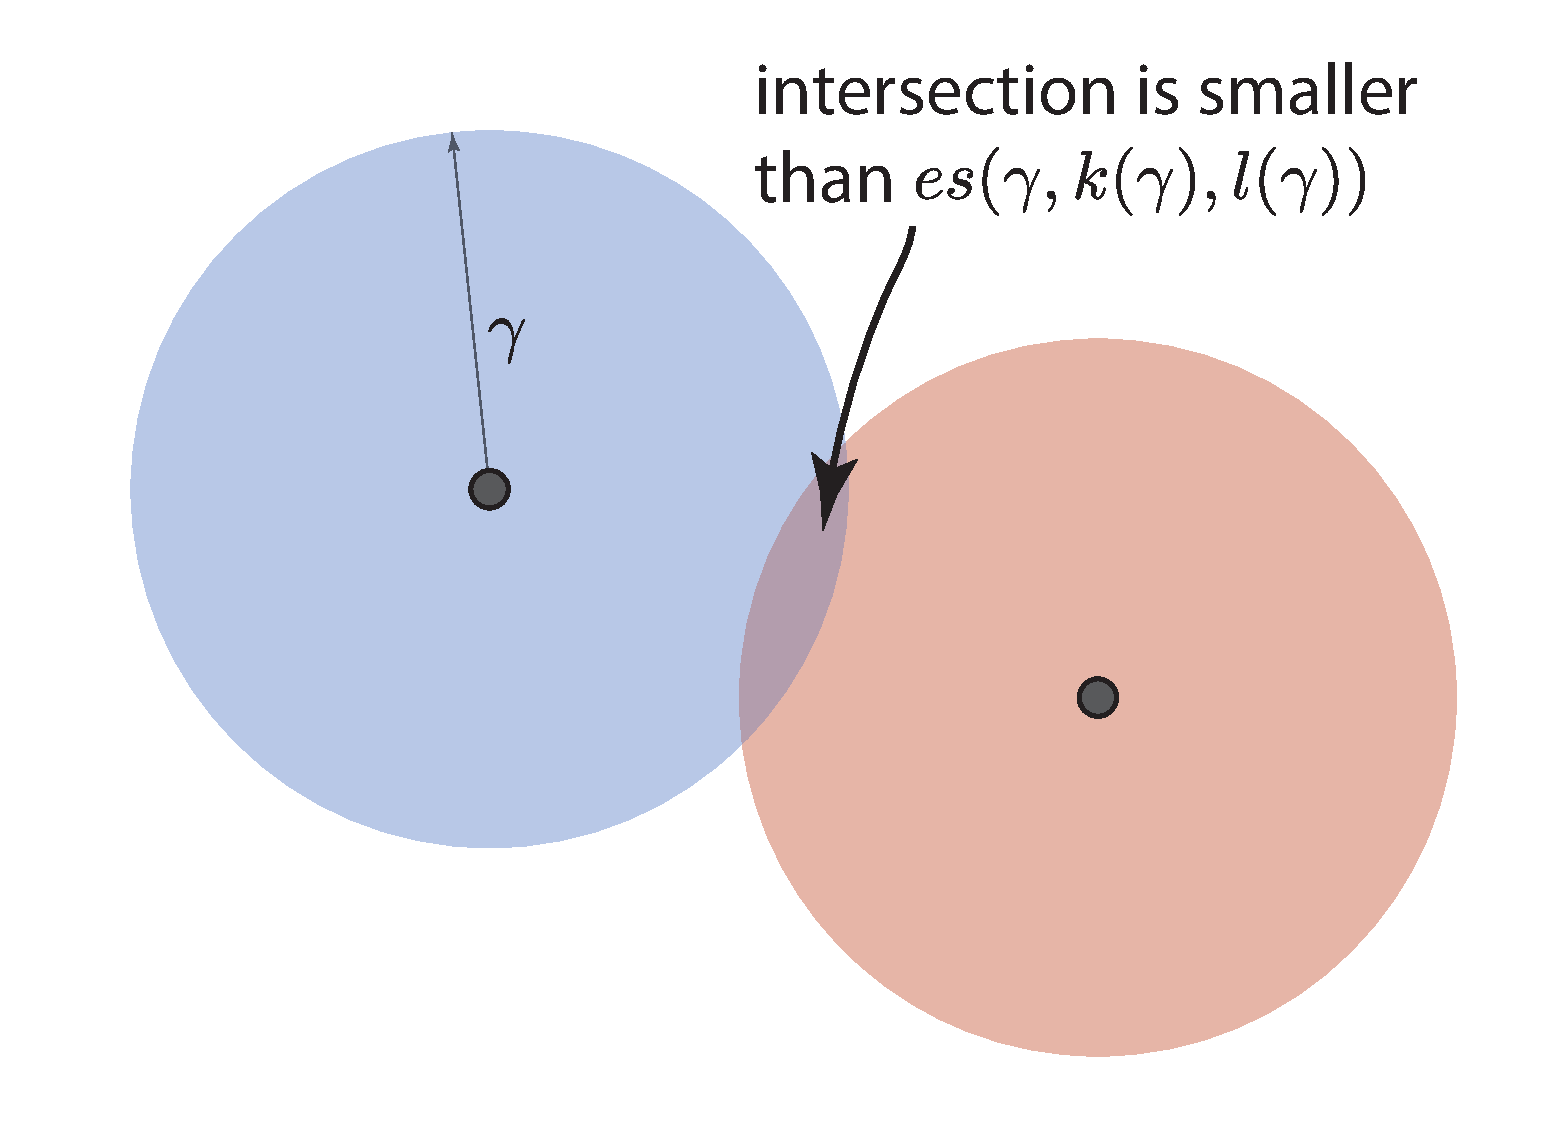
\includegraphics[width=\linewidth]{figures/ch_generic_approach/intersection_due_to_gamma}
      \caption{Two non-similar approximation sets.}
  \end{subfigure}
  \hfill
  \begin{subfigure}[b]{.49\textwidth}
      \label{fig:intersection_due_to_sim}
      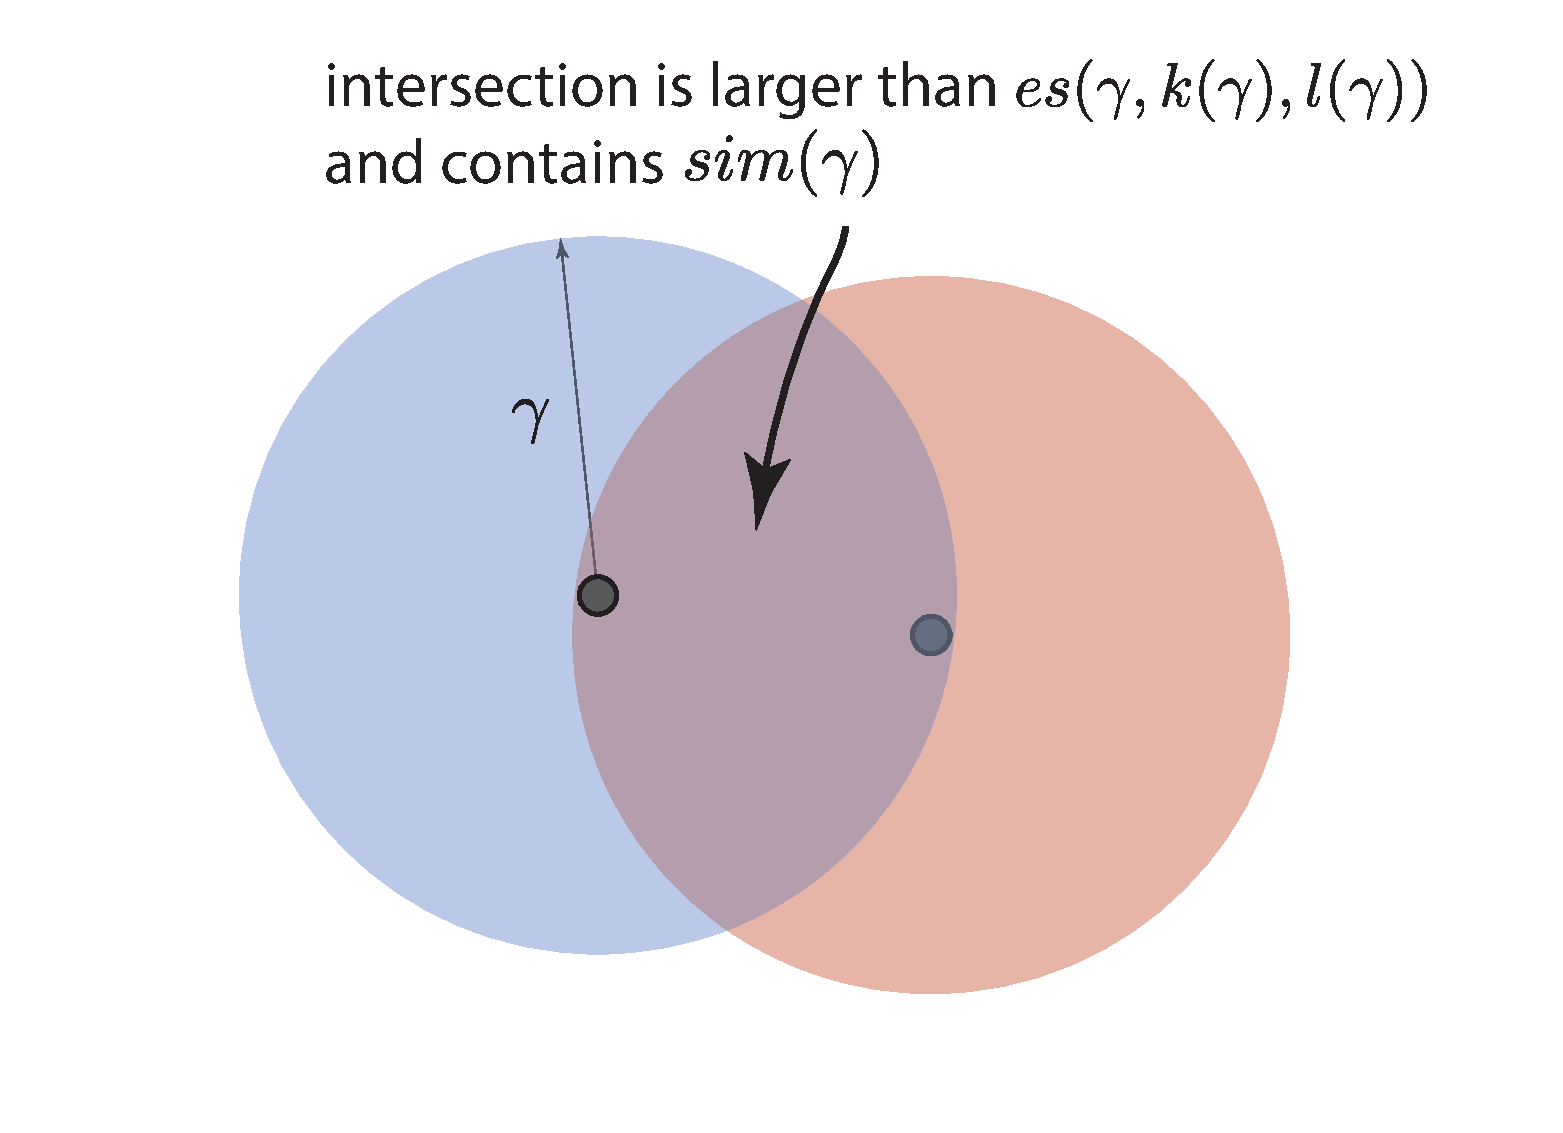
\includegraphics[width=\linewidth]{figures/ch_generic_approach/intersection_due_to_sim}
      \caption{Two similar approximation sets}
  \end{subfigure}
  \\[.5cm]
  \caption{Illustration of ideas contained in Definitions~\ref{def:feasible_as},
  \ref{def:intersection_due_to_gamma} and \ref{def:intersection_due_to_sim}: as
  opposed to randomly chosen approximation sets \textbf{(a)}, two related
  (similar) approximation sets \textbf{(b)} have a $sim(\gamma)$ component of
  the intersection, which we naturally seek to maximize.}
  \label{fig:intersection_types}
\end{figure}

\paragraph{Problem-based instance similarity}
In equation~\eqref{eq:similarity}, the expected size of the intersection is
w.r.t.\  the problem specific probability distribution over all feasible
approximation sets of size $|{\mathcal{C}_\gamma}(X')|$ and
$|{\mathcal{C}_\gamma}(X'')|$, respectively. However, this distribution is hard
to estimate, so,~\citet{Sramek:PhD} introduced a problem-based based instance
similarity, which approximates the denominator by a uniformly chosen pair of
approximation sets.
\index{Similarity approach!Problem-based similarity}
%
\begin{definition}[Problem-based instance similarity]
  Let $X'$ and $X''$ be two input instances of a combinatorial optimization
  problem $\mathcal{P}$ with solution space $\mathcal{C}$. For a given $\gamma$,
  let ${\mathcal{C}_\gamma}(X')$ and ${\mathcal{C}_\gamma}(X'')$ be $\gamma$-approximation sets for $X'$
  and $X''$. Further, let $\mathcal{F}_k$ denote the set of all feasible
  approximation sets of size $k$, i.e., the set of all such sets $F\subseteq
  \mathcal{C}$ of size $k$ for which there exists an instance $I'$ and
  a value $\tilde \gamma$ such that $F=\mathcal{C}_{\tilde \gamma}(\tilde X)$. Then, the expression
  \begin{equation}
    \label{eq:generic_similarity}
    S_\gamma(X',X'') = \frac{|{\mathcal{C}_\gamma}(X')\cap {\mathcal{C}_\gamma}(X'')|}
      {\mathop{\mathbb{E}}_{A\in \mathcal{F}_{|{\mathcal{C}_\gamma}(X')|}, B\in
      \mathcal{F}_{|{\mathcal{C}_\gamma}(X'')|}}{\big[|A\cap B|\big]}}
  \end{equation}
  \nomenclature[D, 03c]{$S_\gamma(X',X'')$}{instance $\gamma$-similarity}%
  \nomenclature[D, 04]{$\mathcal{F}_k$}{all feasible approximation sets}%
  is the \emph{similarity of $X'$ and $X''$ at value $\gamma$} (with respect to
  the optimization problem $\mathcal{P}$), and the expression
  \begin{equation}
    \label{def:S}
    S(X',X'') \coloneqq \max_\gamma S_\gamma(X',X'')
  \end{equation}
  \nomenclature[D, 03d]{$S(X',X'')$}{instance similarity}%
  is the \emph{similarity of $X'$ and $X''$} with respect to the optimization
  problem $\mathcal{P}$.
\end{definition}
%

Thus, the similarity-based approach (in the following referred just as
``similarity'' approach) works as follows. First, we compute the value $\gamma$
that maximizes the similarity
\begin{align}\label{eq:similarity_formula}
  S_\gamma(X',X'') = \frac{|{\mathcal{C}_\gamma}(X')\cap {\mathcal{C}_\gamma}(X'')|}
    {\mathop{\mathbb{E}}_{A\in \mathcal{F}_{|{\mathcal{C}_\gamma}(X')|}, B\in
    \mathcal{F}_{|{\mathcal{C}_\gamma}(X'')|}}{\big[|A\cap B|\big]}},
  \tag{\ref{eq:generic_similarity}}
\end{align}
where the expectation is w.r.t.\ the uniform probability distribution over the
elements in $\mathcal{F}_{|{\mathcal{C}_\gamma}(X')|}$ and $\mathcal{F}_{|{\mathcal{C}_\gamma}(X'')|}$,
respectively. We then return a solution from ${\mathcal{C}_\gamma}(X')\cap {\mathcal{C}_\gamma}(X'')$
uniformly at random.

However, there are two practical issues with the procedure shown above: a)~it is
not always clear how to directly optimize $\gamma$ for the value
of~\eqref{eq:generic_similarity}; and b)~sampling from the intersection of the
corresponding $\gamma$-approximation sets uniformly at random might be
difficult. Despite all that, the similarity approach can be always applied in the 
cases, where one can provide all the steps of Algorithm~\ref{alg:similarity}.

\medskip
\begin{algorithm}[ht!]
\caption{Pipeline for Similarity Approach (Section~\ref{sec:similarity_approach_intro})}
\label{alg:similarity}
  {Determine the domains $\mathcal{F}_k$ of feasible approximation sets of size
  $k$.}

  {Provide a mathematical analysis or an algorithm $ALG_\mathbb{E}$ that
  computes the expected size of the intersection of two approximation sets of
  given sizes $k$ and $l$.}

  {Provide an algorithm $ALG_\cap$ that computes the size of the intersection
  ${\mathcal{C}_\gamma}(X')\cap {\mathcal{C}_\gamma}(X'')$, given $\gamma$ and
  two instances $X'$ and $X''$.}

  {Find $\gamma^*$ that maximizes the similarity $S_\gamma(X',X'')$, using
  $ALG_\mathbb{E}$ and $ALG_\cap$.}

  {Provide an algorithm $ALG_\text{rand}$ that picks a uniform random solution
  from the intersection $\C_{\gamma^*}(X')\cap \C_{\gamma^*}(X'')$.}
\end{algorithm}
\medskip

In order to fulfill these tasks, on can use several tools provided below. It is
important to notice that these useful theorems close the
gap between the ASC formulation~\eqref{eq:asc_mutual_information_formula} and the
similarity approach formulation~\eqref{eq:similarity_formula}.

\begin{theorem}[\citealp{Sramek:PhD}]
  \label{thm:simple}
  Let $\mathcal{P} = (\mathcal{X}, \mathcal{C}, R)$
  (see~Section~\ref{sec:optimization_problem_description}) be an optimization
  problem with the property that for any subset $F$ of the set of all feasible
  solutions $\mathcal{C}$ there exists an instance $\tilde X \in \mathcal{X}$
  and a value $\tilde \gamma$ such that $\mathcal{C}_{\tilde \gamma}(\tilde
  X)=F$. Then, the similarity of two instances $X', X''\in\mathcal{X}$ at value
  $\gamma$ is
  \begin{align}
    \label{eq:simple}
    S_\gamma(X',X'')=\frac{|\mathcal{C}||{\mathcal{C}_\gamma}(X') \cap {\mathcal{C}_\gamma}(X'')|}
      {|{\mathcal{C}_\gamma}(X')||{\mathcal{C}_\gamma}(X'')|}.
  \end{align}
\end{theorem}

However, as \citet{Sramek:PhD} notes, there exists an issue that not every subset
$F\subseteq\mathcal{C}$ is a feasible approximation set, and there is still no general
algorithm of computing the expected size of the intersection. The following
chain of theorems provides some approximation guarantees for the value of~\eqref{eq:simple}.

\begin{theorem}[\citealp{Sramek:PhD}]
  \label{thm:bound}
  Let $\mathcal{P} = (\mathcal{X}, \mathcal{C}, R)$ be an optimization problem. If
  $|{\mathcal{C}_\gamma}(X')|=|{\mathcal{C}_\gamma}(X'')|$ for a given $\gamma$, then
  \begin{align}
    \label{eq:bound}
    S_\gamma(X',X'') \leq \frac{|\mathcal{C}||{\mathcal{C}_\gamma}(X')\cap {\mathcal{C}_\gamma}(X'')|}
      {|{\mathcal{C}_\gamma}(X')||{\mathcal{C}_\gamma}(X'')|}.
  \end{align}
\end{theorem}

\begin{theorem} [\citealp{Sramek:PhD}]
  \label{thm:approx}
  Let $A$ be a constant such that for each feasible solution $c$ of some
  optimization problem $\mathcal{P} = (\mathcal{X}, \mathcal{C}, R)$ it holds that 
  $|\{F\in \mathcal{F}_k | c\in F\}| \leq A k|\mathcal{F}_k|/|\mathcal{C}|$. Then,
  \begin{align}
    S_\gamma(X',X'')\geq\frac{|\mathcal{C}||{\mathcal{C}_\gamma}(X')\cap {\mathcal{C}_\gamma}(X'')|}
      {A |{\mathcal{C}_\gamma}(X')||{\mathcal{C}_\gamma}(X'')|}.
  \end{align}
\end{theorem}

\begin{theorem} [\citealp{Sramek:PhD}]
  \label{thm:worst_case}
  Let $\mathcal{P} = (\mathcal{X}, \mathcal{C}, R)$ be an optimization problem.
  Then,
  \begin{align}
    S_\gamma(X',X'')\geq\frac{|{\mathcal{C}_\gamma}(X')\cap {\mathcal{C}_\gamma}(X'')|}{|{\mathcal{C}_\gamma}(X')||{\mathcal{C}_\gamma}(X'')|}.
  \end{align}
\end{theorem}
%

\myremark This shows that the step of deriving the appropriate specific formula or
algorithm to calculate the expected size of the intersection is a necessary
component of the approach, unless it is possible to show that for a concrete
problem the upper bound is sufficient. We will speculate more on that in the
conclusion to this chapter (Section~\ref{sec:gen_appch_conclusion}).

\section{Proof-of-Concept Prototypic Example}
\label{sec:proof_of_concept}

\index{Prototypic example!For ASC}
Previously, in Section~\ref{sec:asc_original}, we introduced a method of
solution regularization by ASC, and later in
Section~\ref{sec:similarity_approach_intro} we gave a thorough overview of an
analogical approach called instance similarity. While they stem from completely
different roots, it can be easily seen that they both aim at choosing an optimal
approximation set width $\gamma$ in a same way. Specifically, we seek to
optimize
\begin{equation}\label{eq:similarity_maximization_objective}
    \gamma^* = \arg \max_{\gamma >0} \frac{|{\mathcal{C}_\gamma}(X') \cap {\mathcal{C}_\gamma}(X'')|}
      {|{\mathcal{C}_\gamma}(X')||{\mathcal{C}_\gamma}(X'')|}
\end{equation}
\myremark Note that this equation is
\textit{not} identical either to its ASC
version~\eqref{eq:asc_mutual_information_formula} or similarity-based
version~\eqref{eq:similarity_formula}, although yielding same optimization goal;
we will briefly revisit the technical differences, like presence of logarithm,
later in the conclusion.

One of the contributions of this thesis is to present an abstract
proof-of-concept model for prototypical combinatorial optimization problems,
which would allow to experimentally the advantages of the approximation set-based 
approaches. We will mostly experimentally investigate how the methods of
Sections~\ref{sec:asc_original} and~\ref{sec:similarity_approach_intro} perform
on this model.

\subsection{The Example Setting and Terminology}
We expect the approximation set-based methods to exceed the performance of other
optimization methods when the set of solutions that have stable cost over all or
most instances is large enough not to be completely hidden in the noise.
%
To highlight the potential of our approach, we consider an uncertain
minimization problem $(\mathcal{X}, \mathcal{C}, R)$ in which the solution space
$\mathcal{C}$ is partitioned into two sets $\sgood$ and $\sbad$ of sizes $\g$
and $\b$, respectively, which contain the \good\ and the \bad\ solutions,
respectively. Without loss of generality we assume that
\begin{align}
  \C &= \{c_i\}_{i=1}^n \notag \\
  \sgood &= \{c_1,\ldots, c_{|\g|}\} \notag \\
  \sbad &= \{c_{|\g|+1},\ldots,c_{|\g|+|\b|}\}.
\end{align}
\nomenclature[D, 04a]{$\sgood$, $\sbad$}{\good\ and \bad\ solutions}%
%
The sets $\sgood$ and $\sbad$ represent solutions which are desirable and
non-desirable to be chosen, which reflects the fact that the approximation
set-based approaches are designed to reliably tell them apart. We further assume
that $\g \ll \b$, which corresponds to the fact that \good\ solutions should be hard
to identify.

Our proof-of-concept scenario abstracts from a concrete optimization problem. In
other words, we do not address here the problem of specific optimization
algorithms. Hence we explicitly state that instead of generating inputs $X \in
\mathcal{X}$, we rather directly generate costs of solutions $c \in \C$.
%
In the terminology of Section~\ref{sec:optimization_problem_description}, an
instance $X$ can be represented as a vector of random solution costs of length
$n$:
\begin{equation}\label{eq:generic_appch_cost_vector}
  X \coloneqq \langle R_i \rangle_{i=1}^{n},
\end{equation} 
and the cost function is simply
\begin{equation}
  R(c_i, X) \coloneqq R_i,
\end{equation} 
i.e.~the $i$-th entry stores the cost of the solution $c_i$ in $X$.

\subsection{Problem Generation}
\label{sec:gen_appch_pg}

We define the solution ``desirability'' by the intuition that costs of \good\
solutions have a small standard deviation and play the role of signal,
while costs of \bad\ solutions have a higher mean and/or a higher standard
deviation and play the role of deceiving noise.

We assume the cost vector of an instance $X$ to be generated with the following
random problem generating process $PG(\cdot)$:
\begin{itemize}
  \item[1)] the first $\g$ values are chosen at random according to some
            (fixed) probability distribution $\DG$, and
  \item[2)] the remaining $\b$ values are chosen at random according to some
            (fixed) probability distribution $\DB$.
\end{itemize}
\nomenclature[D, 04b]{$\DG$, $\DB$}{cost distributions\nomnorefeq}%

\begin{figure}[t!]
  \centering
  \begin{subfigure}[b]{.8\textwidth}
      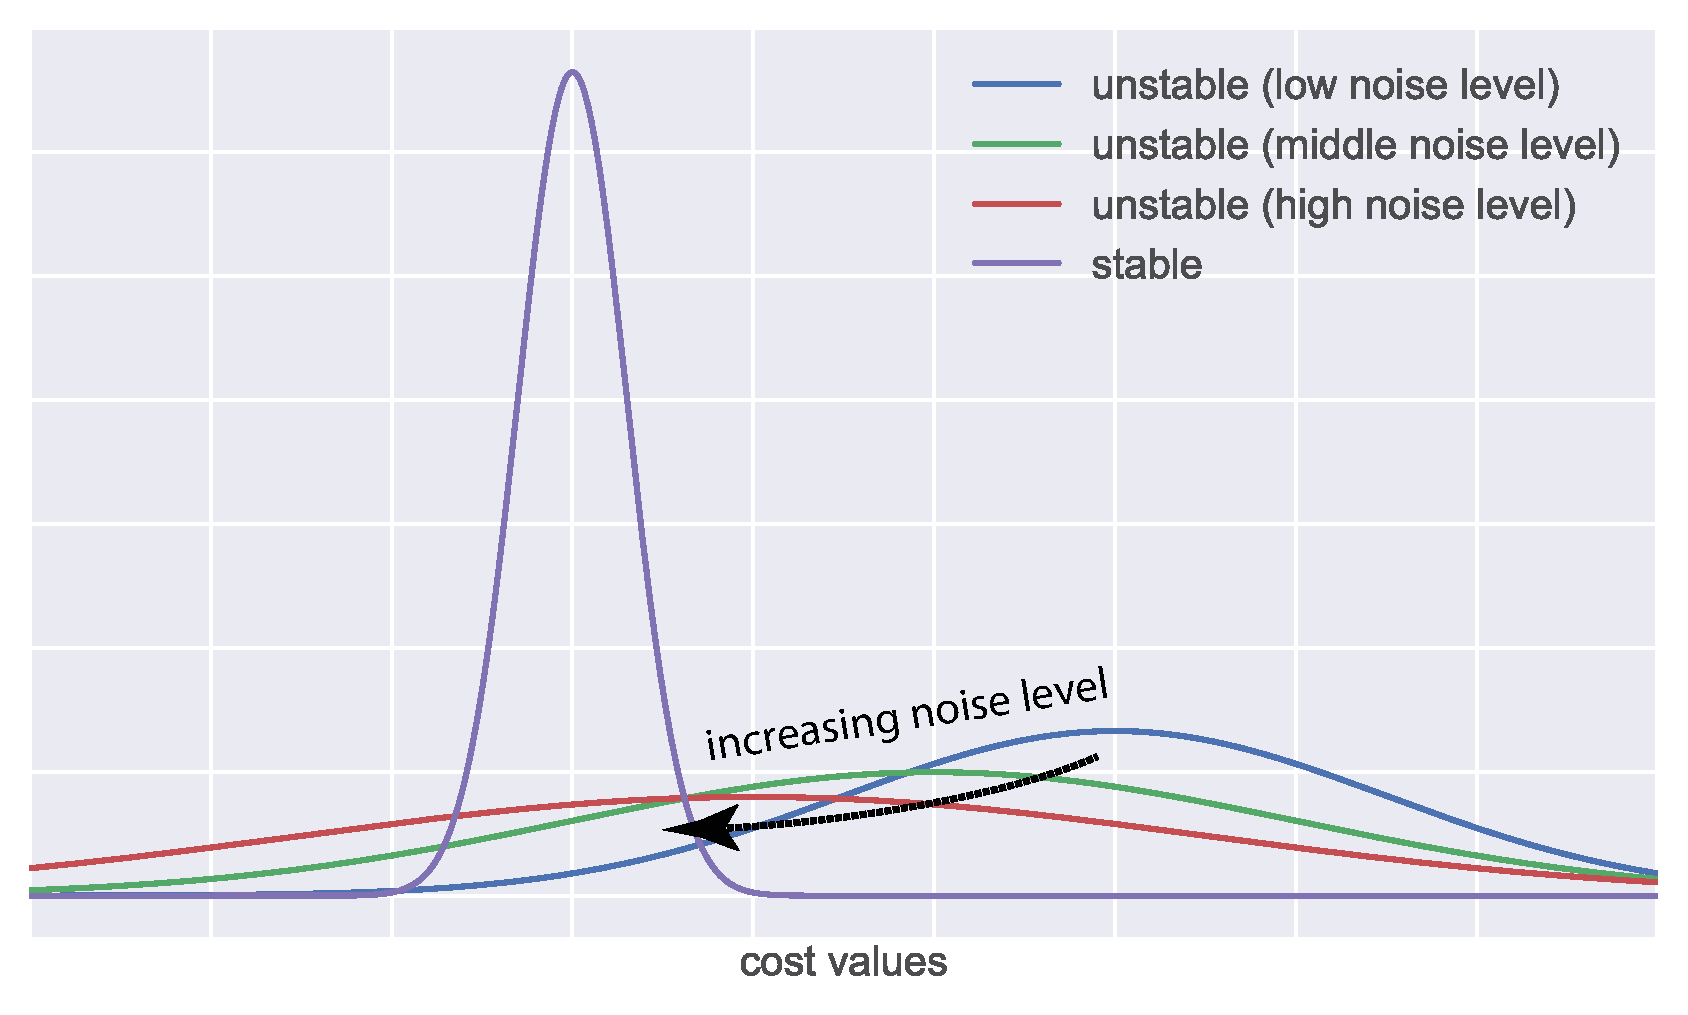
\includegraphics[width=\linewidth]{figures/ch_generic_approach/stable_and_unstable_distr}
  \end{subfigure}
  \caption{Schematic example of \good\ and \bad\ cost distributions and noise
  levels $N \in \mathcal{N}$ of \bad\ ones, as described in
  Section~\ref{sec:gen_appch_pg}.}
  \label{fig:stable_and_unstable_solutions}
\end{figure}

Naturally it is safe to assume that both $\DG$ and $\DB$ have the property that
\good\ solutions are superior to \bad\ ones
(Figure~\ref{fig:stable_and_unstable_solutions}), e.g., because they have a
smaller expected cost or a smaller variance, i.e. for any $R_\text{\good} \sim
\DG$ and $\R_\text{\bad} \sim \DB$, $\Expct [R_\text{\good}] < \Expct [R_\text{\bad}]$ 
and $\Var [R_\text{\good}] < \Var [R_\text{\bad}]$.
We further assume $\DG$ and $\DB$ are independent of the
instance and of the concrete solution (costs of \good\ solutions are always
chosen from $\DG$, costs of \bad\ solutions are always chosen from $\DB$).

We model noise in a generic way by defining a set of noise levels $\mathcal{N}$
(the concrete definition depends on the type of the noise, see~\citep{jcss:2017}). For a fixed noise
level $N\in\mathcal{N}$, we randomly generate an instance as follows. \Good\
solutions are drawn from a distribution with fixed mean $\mu_\mathrm{\G}$ and fixed
standard deviation $\sigma_\mathrm{\G}$.
\Bad\ solutions are drawn from a distribution with mean $\mu_\mathrm{\B}(N)$ and standard
deviation $\sigma_\mathrm{\B}(N)$. The distributions of the \bad\ solutions are
chosen in a way such that for every two noise levels $N,N'\in\mathcal{N}$ with
$N'>N$, we have $\mu_\mathrm{\B}(N')<\mu_\mathrm{\B}(N)$ or
$\sigma_\mathrm{\B}(N')>\sigma_\mathrm{\B}(N)$.
\nomenclature[D, 04c]{$N \in \mathcal{N}$}{noise levels for experiment\nomnorefeq}%

\myremark Such assumptions on noise levels are justified by the fact that noise
would naturally imply either a smaller expected cost, or a higher standard
deviation, or both~--- resulting in a more aggressive ``deceiving'' of the
algorithm. See Figure~\ref{fig:stable_and_unstable_solutions} for schematic
illustration of this intuition.

Due to its enormous theoretical and practical relevance, we present here the
results for the Gaussian noise model (for more noise settings, see~\citep{jcss:2017}).
 \Good\ solutions are drawn from a Gaussian
distribution with mean $\mu_{\G}=1$ and standard deviation $\sigma_{\G}=1$. We
define the noise levels $\mathcal{N}$ in such a way that for each noise level
$N\in\mathcal{N}$, \bad\ solutions are drawn from a Gaussian distribution with
mean $\mu_{\B}(N)=10$ and standard deviation $\sigma_{\B}(N)=N$: $\DG = \mathrm{Norm}(1, 1)$ and
$\DB(N) = \mathrm{Norm}(10, N^2)$.

\subsection{The Goal and Success Metrics}

Now, our goal is the following: given two instances $X'$ and $X''$ generated by
the random process $PG(\cdot)$ described above, our algorithm $\mathscr{A}$ has
to compute a set of solutions $\hat \C_\mathscr{A}$ of candidates for solutions in
$\sgood$, from which it then picks a solution
uniformly at random. The only knowledge of an
algorithm consists of the two cost vectors of $X'$ and $X''$ defined
in~\eqref{eq:generic_appch_cost_vector}. The algorithm cannot exploit the fact
that there are two categories of solutions, and in particular it has no
knowledge about $\DG$ and $\DB$.

Since we assume that a solution from $\hat{\mathcal{C}}_{\mathscr{A}}$ is
picked uniformly at random, we define the \emph{success probability} of $\mathscr{A}$
with input $X'$ and $X''$ as
\begin{align}
  \label{eq:uncert:prob_succ}
  P_{\mathscr{A}}(X',X'')
    = \frac{|{\mathcal{C}}_\mathscr{A}\cap\sgood|}{|{\mathcal{C}}_\mathscr{A}|}
      \text{, for a solving algorithm } \mathscr{A}.
\end{align}
\nomenclature[D, 04d]{$P_{\mathscr{A}}(X',X'')$}{success metric for experiment}%

We want to investigate how the success probabilities of the similarity algorithm
proposed in this chapter evolves with increasing noise, and benchmark it against
some other algorithms. In this thesis, we present only a Joint Minimizer algorithms
(see next section), but for the results produced on a more complete list of benchmarks
we refer the reader to~\citep{jcss:2017}.

\subsection{Experimental Results}
\label{sec:continuous_noise}

\paragraph{Benchmark: joint cost minimizing}
When only two instances are given, the most efficient and straightforward idea
to find a solution that is likely to be good for a test instance is to compute
a solution~$c$ that minimizes the average cost, or equivalently, the joint cost
$R(c, X')+R(c, X'')$. We refer to this method as the \textit{Joint Minimizer}
method in the plots below.
\index{Joint cost minimizer}
\index{Joint minimizer|see{Joint cost minimizer}}

\paragraph{Results}

For each noise level $N\in\mathcal{N}$, we perform the following
experiment: we generate $\R=1000$ instance pairs $(X',X'')_{k\in\{1,\ldots,
\R\}}$ with noise level $N$ according to the $PG(\cdot)$ process described in
Section~\ref{sec:gen_appch_pg}, and for each of these instance pairs we compute
$P_\mathscr{A}(X',X'')$ for all algorithms $\mathscr{A}$. After that we set
\begin{align}
  \hat P_\mathscr{A}(N) &\coloneqq \frac{1}{\R} \sum_{k=1}^{\R} P_\mathscr{A}(X',X'')
\end{align}
to estimate the average success probability of the proposed methods in
dependency of the noise level $N$. Unless otherwise stated, $\mathcal{C}$
contains $n=1000$ solutions.

In our experiments, $\R=1000$ repetitions turned out to be enough to exhibit
the behaviors of the methods. Preliminary experiments with $10000$ repetitions
gave similar results: the rankings of the methods were the same, only the curves in
the plots appeared to be smoother.

Figure~\ref{fig:gnm} shows that the experimental results for
Gaussian noise show a strong indication that the approximation set-based similarity
approach is very competitive against the joint cost minimization.
\begin{figure}[t!]
  \centering
  \begin{subfigure}[b]{.49\textwidth}
      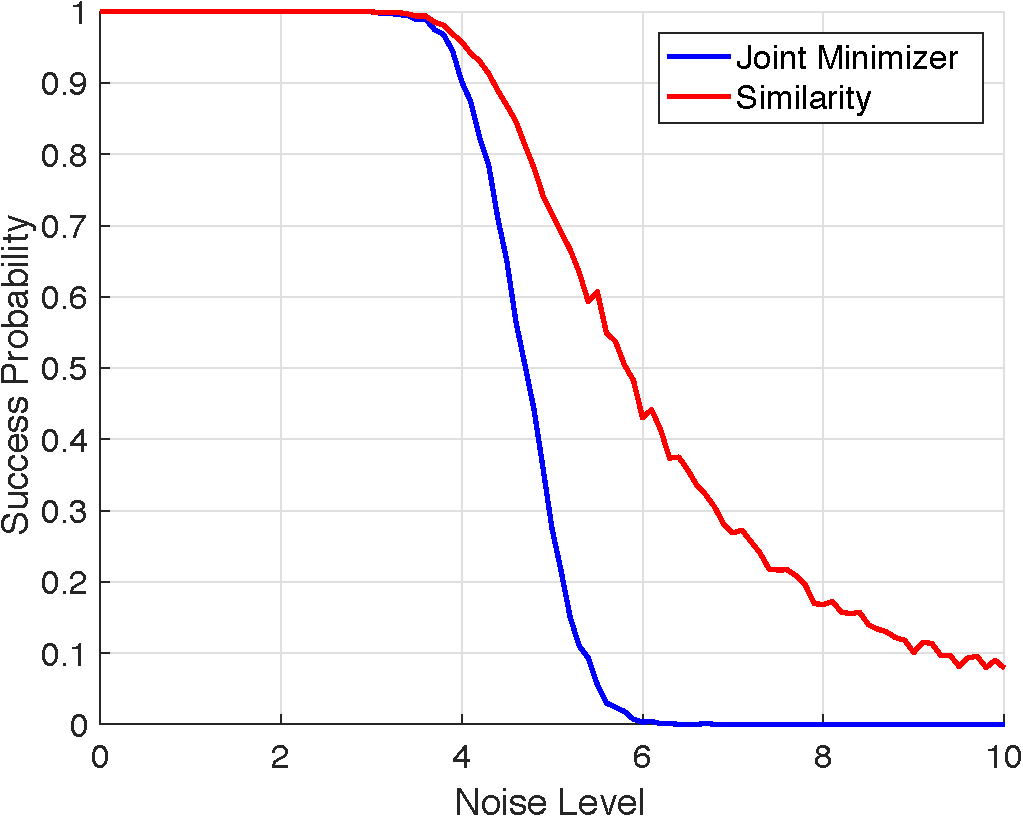
\includegraphics[width=\linewidth]{figures/ch_generic_approach/gnm_g50_b950}
      \caption{$5\%$ of solutions are \good.}
      \label{fig:gnm_5}
  \end{subfigure}
  \hfill
  \begin{subfigure}[b]{.49\textwidth}
      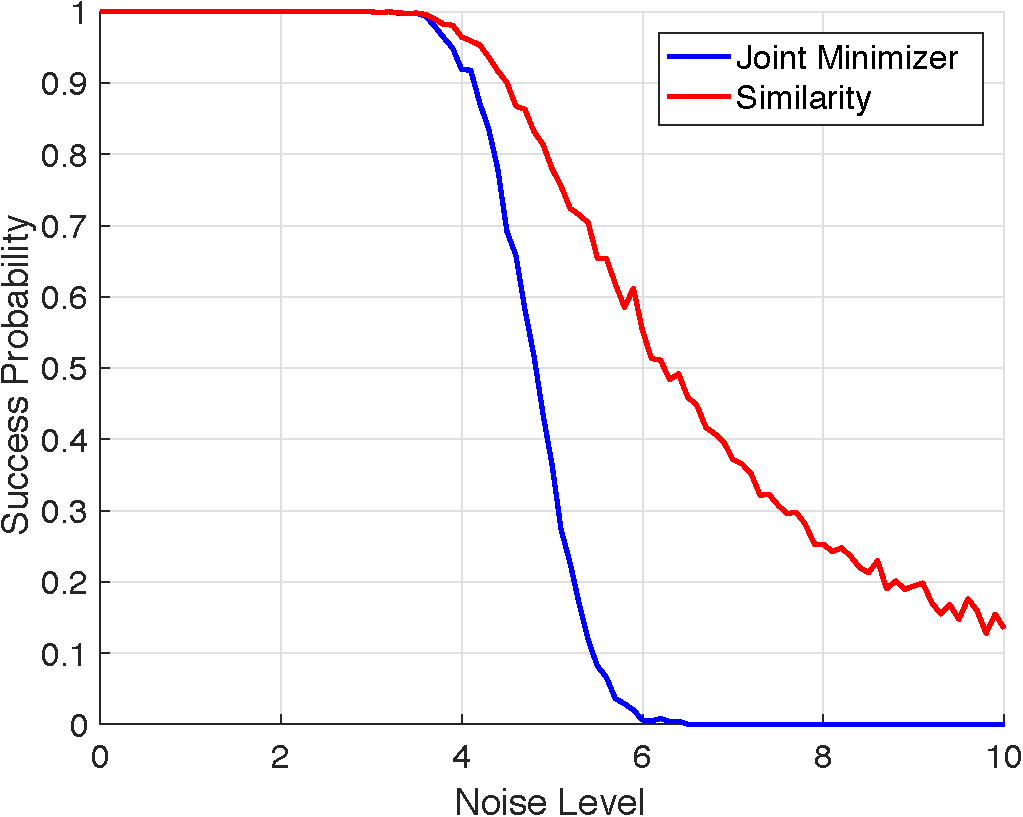
\includegraphics[width=\linewidth]{figures/ch_generic_approach/gnm_g100_b900}
      \caption{$10\%$ of solutions are \good.}
      \label{fig:gnm_10}
  \end{subfigure}
  \\[.5cm]
  \begin{subfigure}[b]{.49\textwidth}
      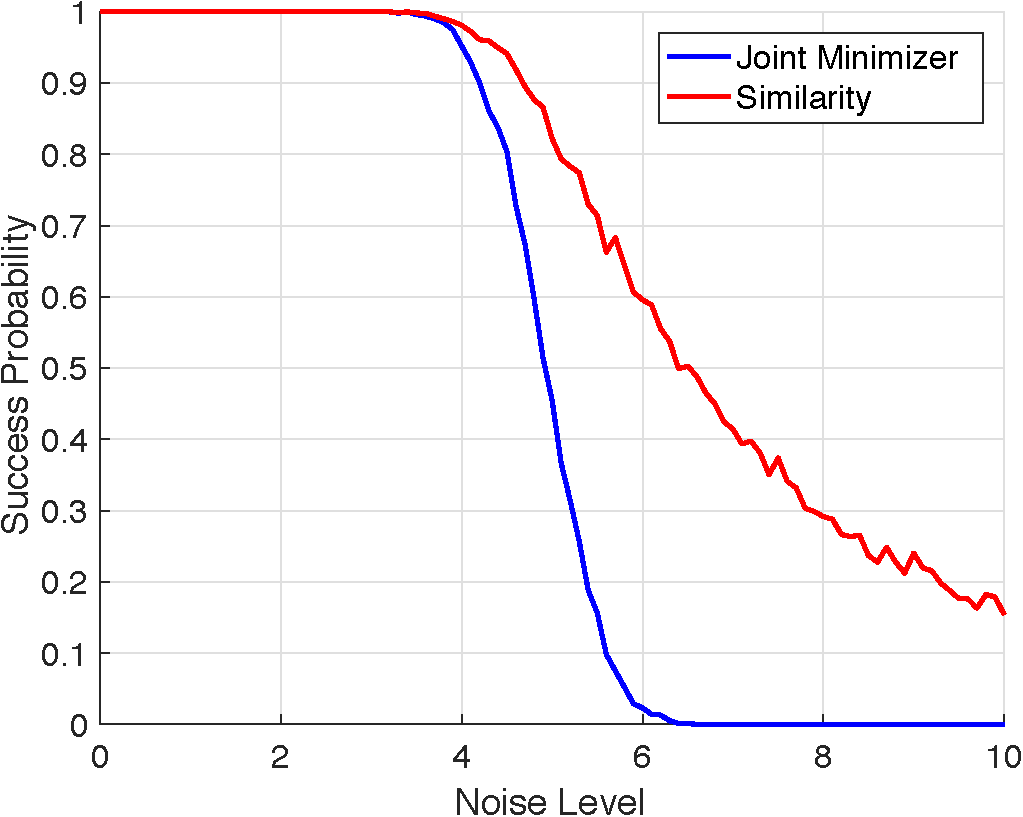
\includegraphics[width=\linewidth]{figures/ch_generic_approach/gnm_g200_b800}
      \caption{$20\%$ of solutions are \good.}
      \label{fig:gnm_20}
  \end{subfigure}
  \hfill
  \begin{subfigure}[b]{.49\textwidth}
      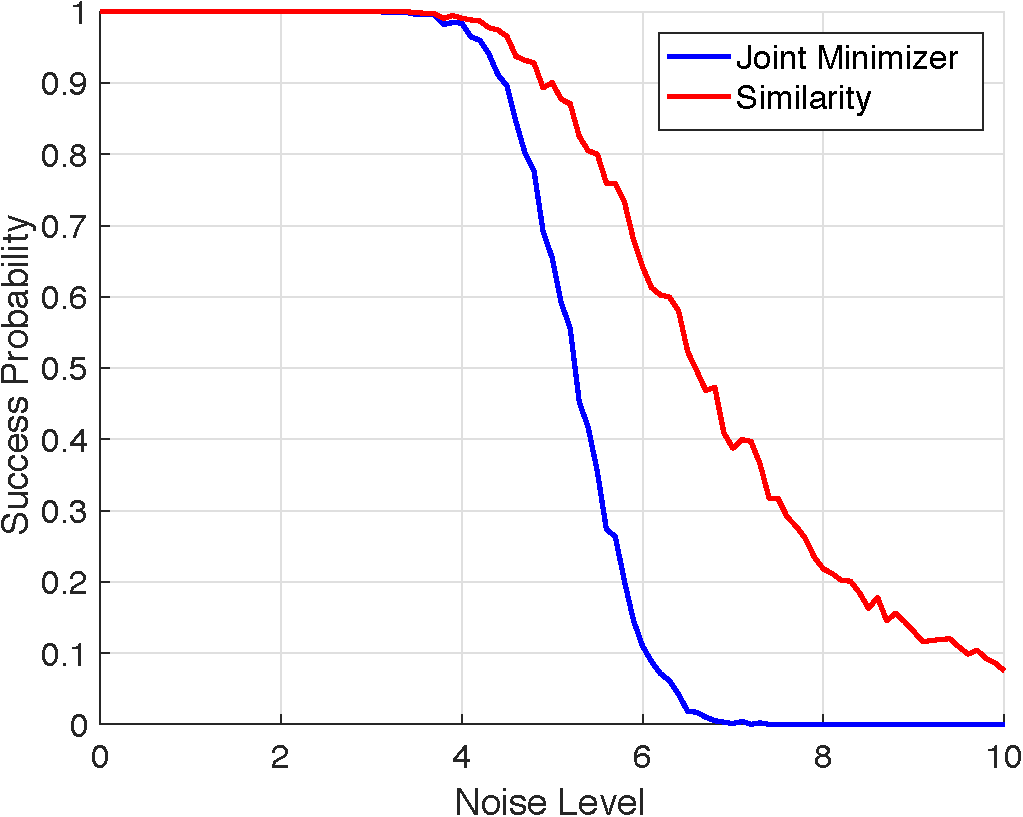
\includegraphics[width=\linewidth]{figures/ch_generic_approach/gnm_g500_b500}
      \caption{$50\%$ of solutions are \good.}
      \label{fig:gnm_50}
  \end{subfigure}
  \\[.5cm]
  \caption{Experimental results where $5\%$ \textbf{(a)}, $10\%$ \textbf{(b)},
    $20\%$ \textbf{(c)} and $50\%$ \textbf{(d)} of the solutions are \good.
    Total number of solutions equals $1000$.}
  \label{fig:gnm}
\end{figure}
Note that the latter is a straightforward way to compute solutions, when only two
inputs are provided. 

\section{Finding Optimal Approximations Analytically}
\label{sec:analytic_solution}

\subsection{Theoretical Results}

One of our main assumptions was that the noise generating process is unknown to
the predicting algorithm $\mathscr{A}$. It was also previously noted that the
crucial step of the whole approximation set-based approach consists in deriving
the appropriate specific formula or algorithm to calculate the
similarity~\eqref{eq:simple}. As a first step towards a formal analysis of the
model discussed in the previous section, in this section we thoroughly
investigate how the similarity~\eqref{eq:simple} behaves in expectation (where
the expectation is computed over all pairs of instances generated by the random
process $PG(\cdot)$), i.e., we analyze the function
\begin{equation}
  \label{eq:oracle_similarity}
  S_\gamma^{\mathrm{EXP}}=\mathbb{E}_{X',X''\sim PG} \,
    S_\gamma(X',X'').
\end{equation}
\index{Similarity approach!Calibration assumption}
\index{Calibration assumption|see{Similarity approach}}
For simplicity we introduce the \emph{calibrating assumption} that the minimum
solutions of both instances $X'$ and $X''$ have the same cost $m$:
\begin{equation}\label{eq:gen_appch_calibrating_assumption}
  \min_c R(c, X') \approx \min_c R(c, X'') \approx m.
\end{equation} 
Without this assumption our analysis would still be possible, but it would be
more technical. Notice that the assumption does not imply that the minimum
solutions themselves are the same: in general, it holds that
\begin{equation}
   \arg \min_c R(c, X') \ne \arg \min_c R(c, X''),
\end{equation} 
i.e. minimum costs are not necessarily attained on the same solution.

\index{Similarity approach!Theoretical estimator}
\begin{theorem}
\label{thm:oracle_similarity}
Let $\gamma>0$, $V = |\mathcal{C}_\gamma(X')\cap \mathcal{C}_\gamma(X'')|$,
$W = |\mathcal{C}_\gamma(X')|\cdot |\mathcal{C}_\gamma(X'')|$, $m$ be the minimum cost of a
solution in both $X'$ and $X''$ (i.e., the calibrating assumption is
satisfied), and $\FG$ and $\FB$ denote the cumulative density functions of the
\good\ and the \bad\ solutions, respectively, evaluated at $m+\gamma$. Then, the
expected similarity~\eqref{eq:oracle_similarity} can be approximated by the
estimated similarity
\begin{align}
  \label{eq:esim}
  S_\gamma^{\mathrm{EXP}} \sim \hat S_\gamma \coloneqq |\mathcal{C}|\left(
    \frac{\Expct[V]}{\Expct[W]} -
    \frac{\Cov(V,W)}{\Expct[W]^2} + \frac{\Var[W] \cdot \Expct[V]}{\Expct[W]^3}\right)
\end{align}
\nomenclature[D, 05]{$S_\gamma^{\mathrm{EXP}}$, $\hat S_\gamma$}{theoretical estimator of similarity}%
where
\begin{align}
  \label{eq:esim:ev}
  \Expct[V] &= \g\FG^2 + \b\FB^2, \\
  \label{eq:esim:ew}
  \Expct[W] &= (\g\FG + \b\FB)^2, \\
  \label{eq:esim:cov}
  \Cov(V, W) &= \g\FG^2(1 - \FG^2) + 2\g(\g-1) \FG^3(1 - \FG) \notag \\
    &\quad + 2\g\b\FG^2\FB (1 - \FG) + 2\g\b\FG\FB^2(1 - \FB) \notag \\
    &\quad + \b\FB^2(1 - \FB^2) + 2\b(\b-1) \FB^3(1 - \FB), \text{ and} \\
  \label{eq:esim:var}
  \Var[W] &= \g^2\FG^2(1- \FG^2) + 2\g^2(\g-1)\FG^3(1 - \FG) \notag\\
    &\quad + 2\g\b(\b - 1) \FG \FB^2 (1 - \FG) \notag\\
    &\quad + 2\g(\g - 1)\b \FG^2 \FB (1 - \FB) \notag\\
    &\quad + 2\g\b \FG \FB (1 - \FG\FB) \notag\\
    &\quad + \b^2 \FB^2 (1 - \FB^2) + 2\b^2(\b-1) \FB^3 (1 - \FB) \notag\\
    &\quad + 4 \g^2 \b \FG^2 \FB (1 - \FG) + 4\g\b^2 \FG \FB^2 (1 - \FB).
\end{align}
\end{theorem}

\paragraph{Proof of Theorem~\ref{thm:oracle_similarity}}
To make this proof more readable, we break it down into several
steps.
\begin{itemize}
  \item[1)] {\em Preliminaries.}
    Let $m=\min_{c \in \mathcal{C}} R(c, X')=\min_{c \in \mathcal{C}} R(c, X'')$. Let
    $c_i$, $i\in\{1,\ldots,\g\}$ denote the solutions in $\sgood$ and
    $\bar c_i$, $i\in\{1,\ldots,\b\}$ denote the solutions in $\sbad$. We define
    \begin{align*}
      A'_{i, \gamma} &= \mathbbm{1}\{R(c_i,X') \le m+\gamma\}, \quad 1 \le i \le \g \\
      A''_{i, \gamma} &= \mathbbm{1}\{R(c_i,X'') \le m+\gamma\}, \quad 1 \le i \le \g \\
      B'_{j, \gamma} &= \mathbbm{1}\{R(\bar c_j,X') \le m+\gamma\}, \quad 1 \le j \le \b \\
      B''_{j, \gamma} &= \mathbbm{1}\{R(\bar c_j,X'') \le m+\gamma\}, \quad 1 \le j \le \b.
    \end{align*}
    \nomenclature[A, 00]{$\mathbbm{1}\{\cdot\}$}{indicator function\nomnorefeqpage}%
    Now the components of the similarity~\eqref{eq:similarity} can be
    expressed as
    \begin{align*}
      |\mathcal{C}_\gamma(X')\cap \mathcal{C}_\gamma(X'')|
        &= \sum_{i = 1}^{\g} A'_{i,\gamma} A''_{i,\gamma} +
          \sum_{j = 1}^{\b} B'_{j,\gamma} B''_{j,\gamma}, \\
      |\mathcal{C}_\gamma(X')|
        &= \sum_{i = 1}^{\g} A'_{i,\gamma} + \sum_{j = 1}^{\b} B'_{j,\gamma}, \\
      |\mathcal{C}_\gamma(X'')|
        &= \sum_{i = 1}^{\g} A''_{i,\gamma} + \sum_{j = 1}^{\b} B''_{j,\gamma}.
    \end{align*}
    For the rest of this proof we will simplify the notation as follows:
    1)~$\gamma$~is omitted in the subscript because we can assume it to be
    the same throughout all considerations, 2) the limits in the sums are
    omitted; for \good\ solutions we
    always sum up to $\g$ and for \bad\ solutions to $\b$, and 3) by $\FG$ and
    $\FB$ we denote the cumulative density functions of \good\ and \bad\
    distributions, respectively, evaluated at $m+\gamma$:
    \begin{equation}
      \FG \coloneqq \FG(m + \gamma), \qquad \FB \coloneqq \FB(m + \gamma).
    \end{equation}
    Observe that 1) $\Expct[A'_i]=\Expct[A''_i]=\FG$ and $\Expct[B'_j]=\Expct[B''_j]
    =\FB$, 2) the random variables in $\{A'_i\}_i \cup \{A''_j\}_j \cup \{B'_k\}_k
    \cup \{B''_\ell\}_\ell$ are jointly independent, and 3) $(A'_i)^2=A'_i$,
    $(A''_i)^2=A''_i$, $(B'_j)^2=Y_j$ and $(B''_j)^2=Y_j$ because these are
    indicators. Also, remember that for jointly independent indicator random
    variables $Z_1, Z_2, Z_3$ with $\Expct[Z_i] = z_i$ we have
    \nomenclature[B, 00]{$\Expct[\cdot]$}{expected value\nomnorefeqpage}%
    \nomenclature[B, 00]{$\Var[\cdot]$}{variance\nomnorefeqpage}%
    \begin{align}
      \Cov(Z_1, Z_2)
        &= z_1 z_2 (1 - z_1 z_2) \label{eq:ag:covariance_general_2} \\
      \Cov(Z_1 Z_2, Z_1 Z_3 )
        &= z_1 z_2 z_3 (1 - z_1) \label{eq:ag:covariance_general_1}
    \end{align}
  \item[2)] {\em Taylor expansion of the expected similarity.}
    A second-order Taylor approximation of $\Expct[V/W]$ gives
    \begin{align}
      \tag{\ref{eq:esim}}
      \Expct\biggl[\frac{V}{W}\biggl]
        \approx \frac{\Expct[V]}{\Expct[W]} -
        \frac{\Cov(V,W)}{\Expct[W]^2} +
        \frac{\Var[W] \cdot \Expct[V]}{\Expct[W]^3}.
    \end{align}
    Remember that $V$ denotes the size of the intersection while $W$ is the
    product of the approximation set sizes. In the following, we will
    analyze each term of~\eqref{eq:esim} separately.
  \item[3)] {\em Expected values of $V$ and $W$.}
    \begin{align*}
      \tag{\ref{eq:esim:ev}}
      \Expct[V] = \sum_i \Expct[A'_i] \cdot \Expct[A''_i] +
        \sum_j \Expct[B'_j] \cdot \Expct[B''_j] = \g\FG^2 + \b\FB^2.
    \end{align*}
    Taking the independence of the random variables into account, for
    $\Expct[W]$ we obtain
    \begin{align*}
      \tag{\ref{eq:esim:ew}}
      \Expct[W]
        = \Expct\Bigl[\sum_i A'_i + \sum_j B'_j\Bigr] \cdot
          \Expct\Bigl[\sum_i A''_i + \sum_j B''_j\Bigr]
        = ( \g \FG + \b \FB )^2.
    \end{align*}
  \item[4)] {\em Analyzing the covariance of $V$ and $W$.}
    Remember that
    \begin{align}
      V &= \sum_i A'_i A''_i + \sum_i B'_i B''_i, \\
      W &= \sum_{j,k} A'_j A''_k + \sum_{i,j} A'_j B''_k +
        \sum_{j,k} B'_j A''_k + \sum_{j,k} B'_j B''_k,
        \label{eq:ag:w_representation}
    \end{align}
    hence
    \begin{align}
      \Cov(V, W)
        &= \sum_{i,j,k} \Cov( A'_i A''_i, A'_j A''_k ) + \sum_{i,j,k} \Cov( A'_i A''_i, A'_j B''_k ) \notag \\
        &+ \sum_{i,j,k} \Cov( A'_i A''_i, B'_j A''_k ) + \sum_{i,j,k} \Cov( A'_i A''_i, B'_j B''_k ) \notag \\
        &+ \sum_{i,j,k} \Cov( B'_i B''_i, A'_j A''_k ) + \sum_{i,j,k} \Cov( B'_i B''_i, A'_j B''_k ) \notag \\
        &+ \sum_{i,j,k} \Cov( B'_i B''_i, B'_j A''_k ) + \sum_{i,j,k} \Cov( B'_i B''_i, B'_j B''_k )
    \end{align}
    We will now analyze each of the single terms.
    \begin{itemize}
      \item[$\bullet$]
        In the first term $\sum \Cov( A'_i A''_i, A'_j A''_k )$
        only the summands with $j=i$ or $k=i$ are non-zero, hence we
        obtain
        \begin{align}
          \sum_{i,j,k} &\Cov( A'_i A''_i, A'_j A''_k )
             = \sum_i \Cov( A'_i A''_i, A'_i A''_i) \notag \\
            &\hspace{1cm}+ \sum_{i \ne j} \Bigl[ \Cov( A'_i A''_i, A'_i A''_j)
            + \Cov( A'_i A''_i, A'_j A''_i)\Bigr] \notag \\
            &= \sum_i \Cov( A'_i A''_i, A'_i A''_i)
            + 2 \sum_{i \ne j} \Cov( A'_i A''_i, A'_i A''_j), \notag\\
            &= \g \FG^2(1 - \FG^2)+2\g(\g-1) \FG^3 (1 - \FG),
            \label{eq:ag:comp_covariance_4}
        \end{align}
        where the last equality holds due
        to~\eqref{eq:ag:covariance_general_2}
        and~\eqref{eq:ag:covariance_general_1}.
      \item[$\bullet$]
        The next two terms $\sum \Cov( A'_i A''_i, A'_j B''_k )$ and
        $\sum \Cov( A'_i A''_i, B'_j A''_k )$ are equal to each other
        (due to the symmetry of $A'$ and $A''$), so their sum resolves
        to
        \begin{equation}
          2 \sum_{i,k} \Cov( A'_i A''_i, A'_i B''_k )
            \stackrel{\text{\eqref{eq:ag:covariance_general_1}}}{=}
            2 \g \b \FG^2 \FB ( 1 - \FG). \label{eq:ag:comp_covariance_2}
        \end{equation}
      \item[$\bullet$]
        The next two terms $\sum \Cov( A'_i A''_i, B'_j B''_k )$
        and $\sum \Cov( B'_i B''_i, A'_j A''_k )$ are both zero
        due to the independence of $A'_i A''_i$ and $B'_j B''_k$.
      \item[$\bullet$]
        The next two terms $\sum \Cov( B'_i B''_i, A'_j B''_k )$
        and $\sum \Cov( B'_i B''_i, B'_j A''_k )$ can be computed in
        exactly the same way as~\eqref{eq:ag:comp_covariance_2} where
        both $\FG$ and $\FB$ as well as $\g$ and $\b$ are interchanged.
        Hence, their sum equals
        \begin{equation*}
          2 \sum_{i,k} \Cov( B'_i B''_i, B'_i A''_k )
            \stackrel{\text{\eqref{eq:ag:covariance_general_1}}}{=}
            2 \g\b \FG \FB^2 ( 1 - \FB).
        \end{equation*}
      \item[$\bullet$]
        The last term $\sum \Cov( B'_i B''_i, B'_j B''_k )$ is computed
        similar as~\eqref{eq:ag:comp_covariance_4},
        performing the above-mentioned replacements, hence
        \begin{align*}
          \sum_{i,j,k} &\Cov( B'_i B''_i, B'_j B''_k )
            = \b \FB^2(1 - \FB^2) + 2\b(\b-1) \FB^3 (1 - \FB).
        \end{align*}
    \end{itemize}
  \item[5)] {\em Analyzing the variance of $W$.}
    Finally we compute $\Var[W] = \Cov(W, W)$. When $W$ is expressed
    as~\eqref{eq:ag:w_representation}, we obtain
    \begin{align*}
      \Cov(W, W)
      &= \sum_{i,j,k,\ell} \Cov(A'_i A''_j, A'_k A''_\ell) + \sum_{i,j,k,\ell} \Cov(A'_i B''_j, A'_k B''_\ell) \\
      &+\sum_{i,j,k,\ell} \Cov(B'_i A''_j, B'_k A''_\ell) + \sum_{i,j,k,\ell} \Cov(B'_i B''_j, B'_k B''_\ell) \\
      &+ 2 \sum_{i,j,k,\ell} \Cov(A'_i A''_j, A'_k B''_\ell) + 2 \sum_{i,j,k,\ell} \Cov(A'_i A''_j, B'_k A''_\ell) \\
      &+ 2 \sum_{i, j, k, \ell} \Cov(A'_i A''_j, B'_k B''_\ell) + 2 \sum_{i,j,k,\ell} \Cov(A'_i B''_j, B'_k A''_\ell) \\
      &+ 2 \sum_{i,j,k,\ell} \Cov(A'_i B''_j, B'_k B''_\ell) + 2 \sum_{i,j,k,\ell} \Cov( B'_i A''_j, B'_k B''_\ell).
    \end{align*}
    As before we analyze each of these terms separately.
    \begin{itemize}
      \item[$\bullet$]
        The first term $\sum \Cov(A'_i A''_j, A'_k A''_\ell)$ can be
        expressed as
        \begin{align*}
          &\sum_{i} \Cov(A'_i A''_i, A'_i A''_i)
            + 4 \sum_{i\ne j} \Cov(A'_i A''_i, A'_i A''_j) \\
          &+ 2\hspace{-4mm}\sum_{i \ne j, i \ne k, j \ne k}\hspace{-4mm} \Cov( A'_i A''_j, A'_i A''_k)
            + \sum_{i \ne j} \Cov( A'_i A''_j, A'_i A''_j)
        \end{align*}
        where
        \begin{align*}
          \sum_{i} \Cov(A'_i A''_i, A'_i A''_i) &= \g\FG^2(1 - \FG^2), \\
          4 \sum_{i\ne j} \Cov(A'_i A''_i, A'_i A''_j) &= 4\g(\g-1)\FG^3(1-\FG), \\
          2\hspace{-4mm}\sum_{i \ne j, i \ne k, j \ne k}\hspace{-4mm}
              \Cov( A'_i A''_j, A'_i A''_k) &= 2\g(\g-1)(\g-2) \FG^3( 1- \FG), \\
          \sum_{i \ne j} \Cov( A'_i A''_j, A'_i A''_j) &= \g(\g-1)\FG^2 ( 1 - \FG^2),
        \end{align*}
        and therefore
        \begin{equation}
          \label{eq:ag:comp_covariance_6}
          \sum_{i,j,k,\ell}\hspace{-1mm} \Cov(A'_i A''_j, A'_k A''_\ell)
            = \g \FG^2( 1- \FG^2) + 2 \g^2 (\g-1) \FG^3 ( 1- \FG).
        \end{equation}
      \item[$\bullet$]
        The next two terms $\sum \Cov(A'_i B''_j, A'_k B''_\ell)$ and
        $\sum \Cov(B'_i A''_j, B'_k A''_\ell)$ are equal due to the
        symmetry in instances, hence their sum equals
        \begin{align*}
          %&2 \sum_{i, j, k, \ell} \Cov(A'_i B''_j, A'_k B''_\ell) \\
          &2 \sum_{\substack{i \\ j \ne k}} \Cov(A'_i B''_j, A'_i B''_k)
            + 2 \sum_{\substack{i \\ j \ne k}} \Cov(A'_j B''_i, A'_k B''_i) \\
          &\quad + 2 \sum_{i, j} \Cov(A'_i B''_j, A'_i B''_j),
        \end{align*}
        where the the terms are computed as
        \begin{align*}
          2 \sum_{\substack{i \\ j \ne k}} \Cov(A'_i B''_j, A'_i B''_k)
            &\stackrel{\text{\eqref{eq:ag:covariance_general_1}}}{=}
              2 \g\b(\b-1) \FG \FB^2 (1 - \FG), \\
          2 \sum_{\substack{i \\ j \ne k}} \Cov(A'_j B''_i, A'_k B''_i)
            &\stackrel{\text{\eqref{eq:ag:covariance_general_1}}}{=}
              2 \g (\g-1) \b \FG^2 \FB (1 - \FB), \\
          2 \sum_{i, j} \Cov(A'_i B''_j, A'_i B''_j)
            &\stackrel{\text{\eqref{eq:ag:covariance_general_2}}}{=}
              2\g\b \FG \FB ( 1 - \FG \FB).
        \end{align*}
      \item[$\bullet$]
        The next term $\sum \Cov(B'_i B''_j, B'_k B''_\ell)$ is computed
        analogically to~\eqref{eq:ag:comp_covariance_6}
        where \good\ and \bad\ solutions are interchanged, resulting in
        \begin{align*}
          \sum_{i,j,k,\ell} &\Cov(B'_i B''_j, B'_k B''_\ell)
            = \b^2 \FB^2 ( 1 - \FB^2) + 2 \b^2(\b-1) \FB^3 (1 - \FB).
        \end{align*}
      \item[$\bullet$]
        The next terms $2\sum \Cov(A'_i A''_j, A'_k B''_\ell)$ and
        $2\sum \Cov(A'_i A''_j, B'_k A''_\ell)$ are equal due to the
        symmetry of the instances, hence their sum is
        \begin{align}\label{eq:ag:comp_covariance_7}
          4 \sum_{i,j,k,\ell} \Cov(A'_i A''_j, A'_k B''_\ell)
            &= 4 \sum_{i,j,k} \Cov(A'_i A''_j, A'_i B''_k) \notag \\
            &\stackrel{\text{\eqref{eq:ag:covariance_general_1}}}{=} 4 \g^2 \b \FG^2 \FB ( 1 - \FG ).
        \end{align}
      \item[$\bullet$]
        The next terms $2\sum \Cov(A'_i A''_j, B'_k B''_\ell)$ and
        $2\sum \Cov(A'_i B''_j, B'_k A''_\ell)$ are both equal to zero
        due to the independence of $A'_i A''_j$ and $B'_k B''_\ell$, and
        of $A'_i B''_j$ and $A'_k A''_\ell$.
      \item[$\bullet$]
        The last terms $2\sum \Cov(A'_i B''_j, B'_k B''_\ell)$ and
        $2\sum \Cov(B'_i A''_j, B'_k B''_\ell)$ are equal due to the
        symmetry the instances hence their sum can be computed
        analogically to~\eqref{eq:ag:comp_covariance_7} where \good\ and
        \bad\ solutions are interchanged. Hence, we obtain
        \begin{equation*}
          4 \sum_{i,j,k,\ell} \Cov(B'_i A''_j, B'_k B''_\ell)
            = 4 \g \b^2 \FG \FB^2 ( 1 - \FB).
            \qedhere
        \end{equation*}
        \nomenclature[B, 00]{$\Cov(\cdot, \cdot)$}{covariance\nomnorefeqpage}%
    \end{itemize}

\end{itemize}
 
The proof is thus finished.
\QEDA

\subsection{Experimental Results}
We now provide both positive and negative experimental results which highlight
the scope of applicability of such similarity estimation.  We performed an
experimental evaluation using Gaussian noise in a setting similar to the one in
Sections~\ref{sec:gen_appch_pg}--\ref{sec:continuous_noise}: parameters were set
to $\g=100$, $\b=900$, $\mu_{\mathrm{\G}}=1$, $\sigma_{\mathrm{\G}}=1$, $\mu_{\mathrm{\B}}=10$,
$\sigma_{\mathrm{\B}}\in\{0,0.1,\ldots,10\}$.
% 
The only adjustment on had to make was a slightly changed instance generator due
to the calibrating assumption~\eqref{eq:gen_appch_calibrating_assumption}: since
the minima of both instances have to be sufficiently close to each other, the
problem generation process disregarded each pair of instances for which the
minima $m'$ and $m''$ differed by more than $\varepsilon=10^{-4}$, and
repeatedly generated a new pair until $|m'-m''|\le
\varepsilon$. 

For each successful (i.e. not rejected due to calibrating assumption) instance
pair $(X',X'')$, we computed similarity~\eqref{eq:simple} and
estimated similarity~\eqref{eq:esim}, where the latter was calibrated with
$m=(m'+m'')/2$. We repeated the process $\R=1000$ times and calculated the
average similarity
\begin{equation}
  \bar S_\gamma=\frac{1}{\R}\sum_{k=1}^\R S_\gamma(X',X''),
\end{equation}
and compared it to the estimated similarity~\eqref{eq:esim}. We note that we did
not compute the average estimated similarity over all instance pairs, but
instead calibrated Equation~\eqref{eq:esim} directly using the average minimum
cost of the instance pairs, i.e., using $m=\frac{1}{\R}\sum_{k=1}^\R
(m'^k+m''^k)/2$ where $m'^k=\min_{c \in \mathcal{C}} R(c, X'^k)$ and $m''$ is
defined respectively.

Figure~\ref{fig:realVsEstimatedSimilarities} shows the plots of $\hat S_\gamma$ and
$\bar S_\gamma$ defined above for two noise levels: $\sigma_{\mathrm{\B}}=1$ and for $\sigma_{\mathrm{\B}}=5$.
\begin{figure}[ht!]
  \centering
  \begin{subfigure}[b]{.6\textwidth}
      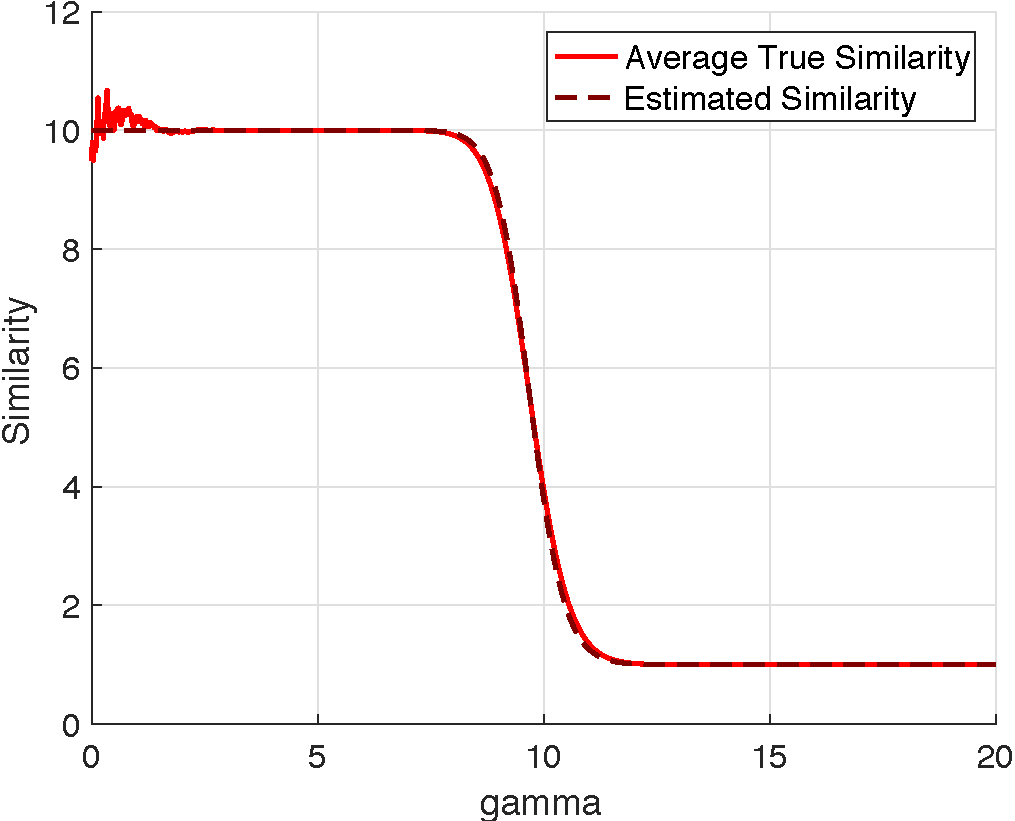
\includegraphics[width=\linewidth]{figures/ch_generic_approach/realVsEstimatedSimilarities_sb1}
      \caption{}
  \end{subfigure}
  \\[.5cm]
  \begin{subfigure}[b]{.6\textwidth}
      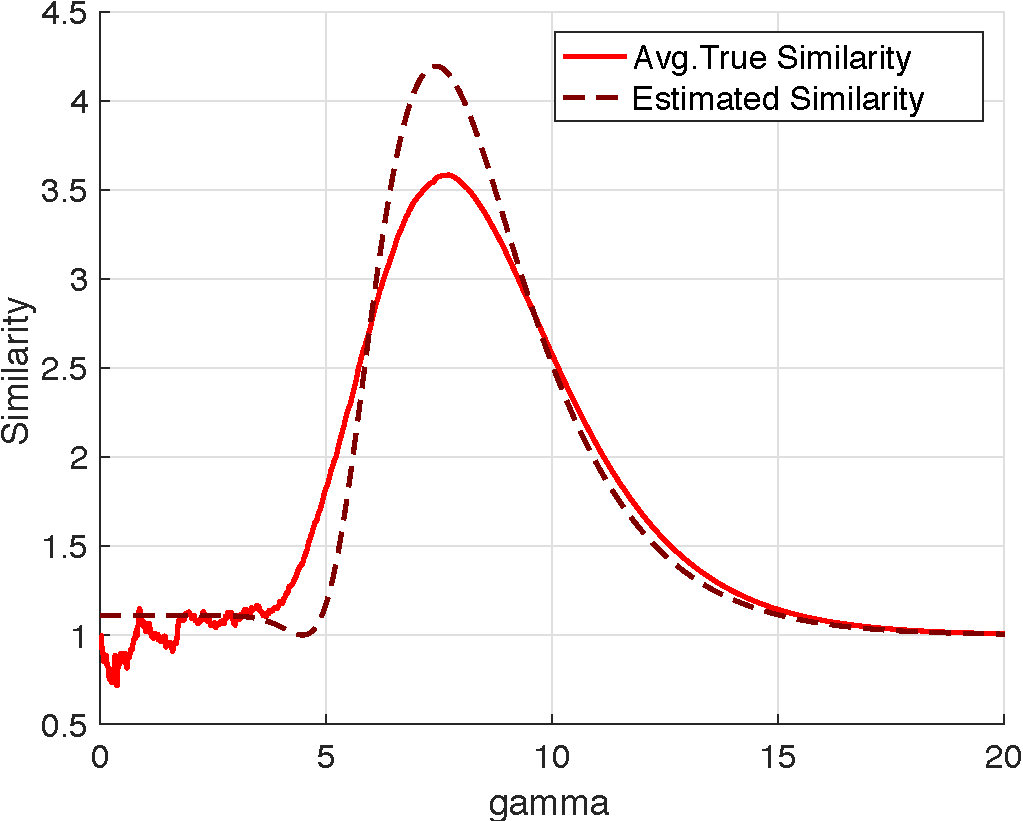
\includegraphics[width=\linewidth]{figures/ch_generic_approach/realVsEstimatedSimilarities_sb5}
      \caption{}
  \end{subfigure}
  \\[.5cm]
  \caption{Average vs. estimated similarity for $\sigma_{\mathrm{\B}}=1$ \textbf{(a)}, and for
    $\sigma_{\mathrm{\B}}=5$ \textbf{(b)}.}
  \label{fig:realVsEstimatedSimilarities}
\end{figure}
We see that the estimated similarity matches the average similarity relatively
well, especially for larger values of $\gamma$. Although the discrepancy grows
with the noise (which is natural due to the Taylor expansion used in the proof),
probably the most important thing to note is that the positions of the $\gamma^*$
computed based on $\hat S_\gamma$ and $\bar S_\gamma$ remain the same.

% \agcomm{till here}

% For $\sigma_{\mathrm{\B}}=5$, the situation is more difficult to analyze. However,
% Figure~\ref{fig:realVsEstimatedSimilarities}b shows that the maximum of the
% estimated similarity is larger than the estimated similarity at $\gamma=0$, and
% it also shows that the values $\gamma$ where the average and the estimated
% similarity, respectively, are maximized coincide well. Therefore the
% aforementioned problem of an empty intersection does not occur.

% As before we computed for both methods the
% intersection $\mathcal{C}_{\gamma^*}(X')\cap \mathcal{C}_{\gamma^*}(X'')$ and
% evaluated the resulting success probability using the definition
% in~\eqref{eq:uncert:prob_succ}. 
% Figure~\ref{fig:realVsEstimated} shows that for
% high noise, \tESIM\ has a higher chance to pick a \good\ solution than \tSIM\
% and \tMR\ which is not surprising because it has knowledge about the underlying
% process.
% \begin{figure}[t!]
%   \centering
%   \begin{subfigure}[b]{.85\textwidth}
%       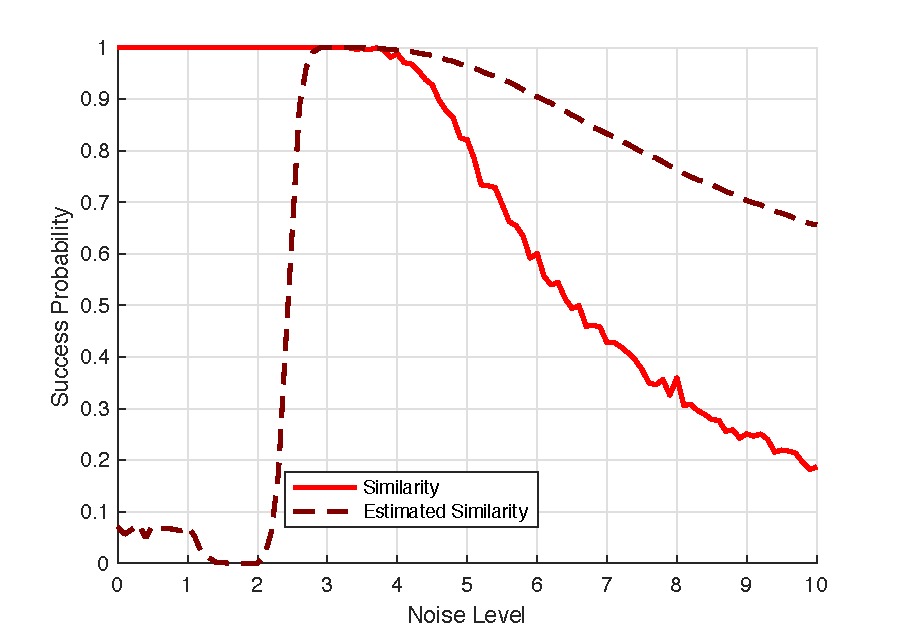
\includegraphics[width=\linewidth]{figures/ch_generic_approach/realVsEstimatedSuccessProbabilities}
%   \end{subfigure}
%   \\[.5cm]
%   \begin{subfigure}[b]{.85\textwidth}
%       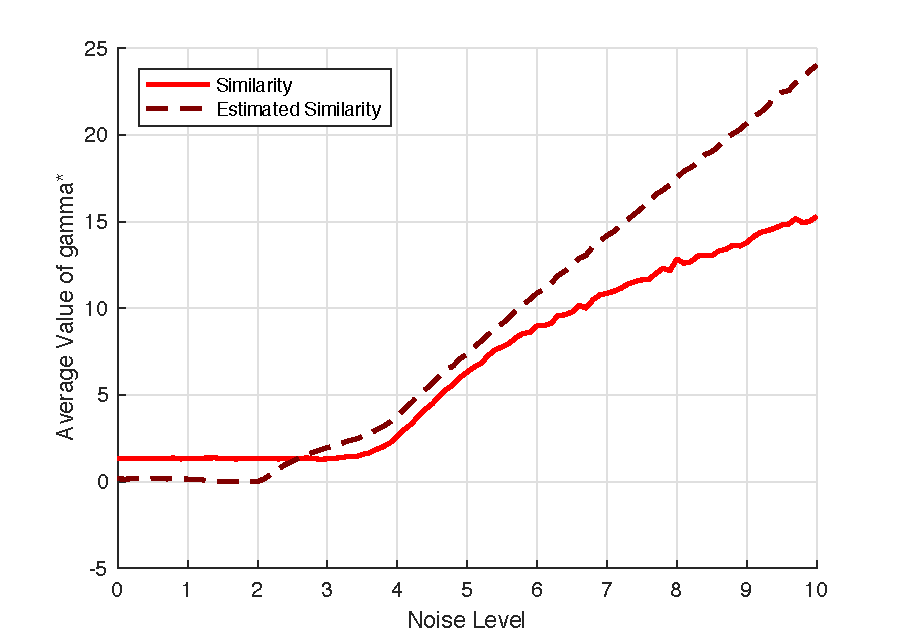
\includegraphics[width=\linewidth]{figures/ch_generic_approach/realVsEstimatedGamma}
%   \end{subfigure}
%   \\[.5cm]
%   \caption{Comparison of the success rates of \tMR\ and \tSIM\ with the one of
%     the estimated similarity (a), and a comparison of the values $\gamma^*$
%     that \tMR, \tSIM\ and \tESIM\ compute.}
%   \label{fig:realVsEstimated}
% \end{figure}

% The weak performance of the estimated similarity for small noise seems to be
% more surprising. To understand why this happens, consider
% Figure~\ref{fig:realVsEstimated}b\AGcomm{Fig ref broken} which shows the average value of $\gamma^*$
% that each method computes. Observe that for $\sigma_{\mathrm{\B}}<2.5$, the average value of
% $\gamma^*$ that the estimated similarity computes is below the one that
% \tMR\ computes, and since \tMR\ computes the
% smallest $\gamma$ for which the intersection of both $\gamma$-approximation sets
% is non-empty, the estimated similarity nearly always underestimates $\gamma$. To
% understand why this happens, we investigate the situation for $\sigma_{\mathrm{\B}}=1$ (low
% noise) and $\sigma_{\mathrm{\B}}=5$ (moderate noise). For each of the $\R=1000$ experiments,
% we compared the values of $\gamma^*$ that \tSIM\ computes with the
% ones of the estimated similarity. Figure~\ref{fig:realVsEstimatedPairs} shows
% the distribution of the points $(\gamma_\SIM^*,\gamma_\ESIM^*)$ where a point is
% red if \tSIM\ outperformed \tESIM, and green
% otherwise.
% \begin{figure}[t]
%   \centering
%   \begin{minipage}[t]{\textwidth}
%     \small
%     \centering
%     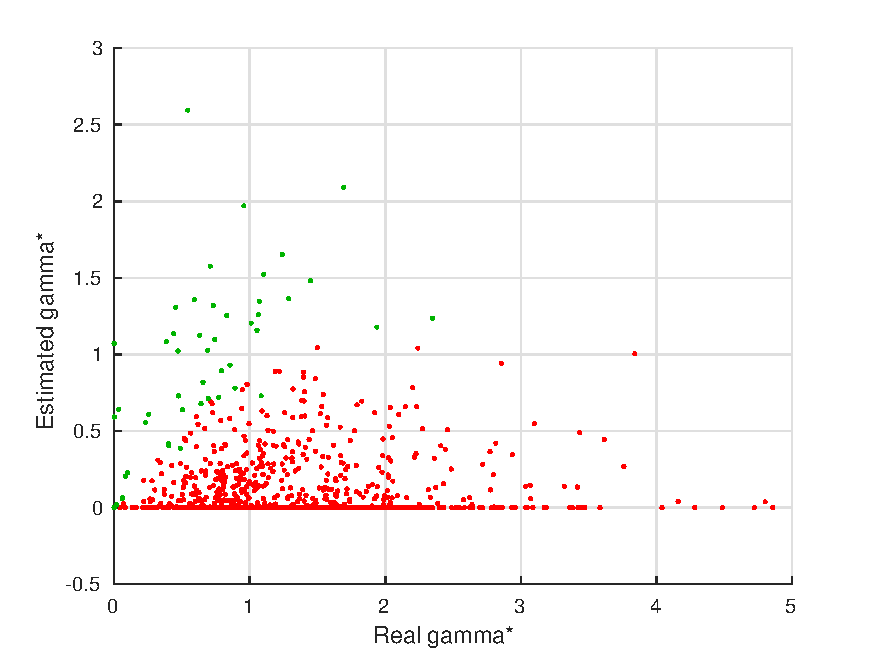
\includegraphics[width=.9\linewidth]{figures/ch_generic_approach/realVsEstimatedGamma_sb1}
    
%     (a)
%   \end{minipage}\\
%   \begin{minipage}[t]{\textwidth}
%     \small
%     \centering
%     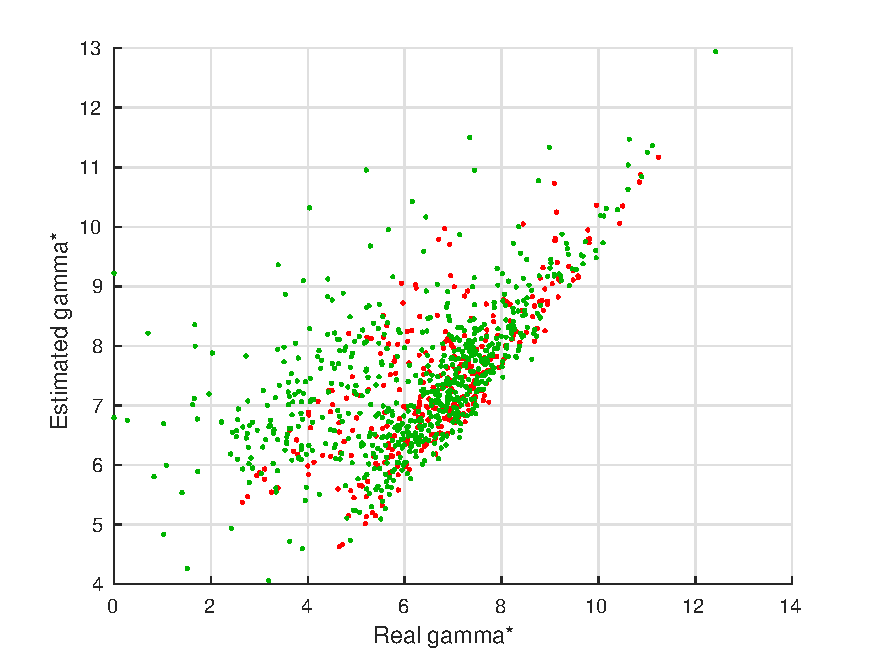
\includegraphics[width=.9\linewidth]{figures/ch_generic_approach/realVsEstimatedGamma_sb5}
    
%     (b)
%   \end{minipage}
%   \caption{Each point corresponds to the outcome of one experiment, where the
%     $x$-coordinate denotes the value $\gamma^*$ computed by \tSIM\ and the
%     $y$-coordinate denotes the value $\gamma^*$ computed by \tESIM. A point
%     is red if \tSIM\ outperformed \tESIM, and green otherwise. The
%     experiments were performed for $\sigma_{\mathrm{\B}}=1$ (a), and for $\sigma_{\mathrm{\B}}=5$
%     (b).}
%   \label{fig:realVsEstimatedPairs}
% \end{figure}
% We see that for low noise, the estimated similarity nearly always
% underestimates $\gamma^*$. On the other hand, the choice of $\gamma^*$ for
% moderate noise is often better than the one by \tSIM. Hence, it
% seems that \tSIM\ is still too much influenced by the noise in the
% instances.

To summarize, we considered the expected similarity of two instances from the
same generator, and we derived an estimation for it that only depends on the
number of \good\ and \bad\ solutions, and on the respective cumulative density
functions. Our experiments showed that our estimation approximates the expected
similarity well when the noise is not too low. 
%
Our experiments also showed that the $\gamma^*$ that maximizes the estimated
similarity does indeed help to identify \good\ solutions. In particular,
choosing a solution from the intersection of the corresponding
$\gamma^*$-approximation is a promising way of robust solving. One of the
possible steps in this direction should be to analyze how many \good\ and how
many \bad\ solutions this intersection contains in expectation.

\section{Gibbs Relaxation of the Approximation Set-Based Approach}
\label{sec:gibbs_relaxation_of_sim}

\subsection{Approximation Sets with Gibbs Weights}
\label{sec:gibbs_relaxation_of_sim_weights}

\index{Approximation Set Coding!Gibbs relaxation}
\index{Gibbs relaxation|see{Approximation Set Coding}}
\nomenclature[D, 06]{$w^G_\beta(c, X)$}{Gibbs weights\nomnorefeq}%
\nomenclature[D, 06a]{$\beta$}{inverse temperature\nomnorefeq}%
\citet{conf/isit/Buhmann10}, in addition to the approximation set-based
approach, introduced its Gibbs-relaxed version which we give in this section.
The idea (we adapt it for the sake of notation alignment with the material of
this chapter) is as follows: using the maximum entropy principle
(Section~\ref{sec:background_max_entropy}) by~\citet{Jaynes82} from statistical
physics~\citep[see also][]{book/MezardM09}, for a real number $\beta \ge 0$, an
instance~$X$ and a solution~$c$, the Gibbs weight \index{Gibbs weights} of $c$
is defined as $w^G_\beta(c, X)
\coloneqq \exp(-\beta R(c, X))$. Now one computes a value $\beta^*$ that
maximizes
\begin{align}
  \label{eq:gibbs_realaxation}
  \beta^* = \arg \max_{\beta > 0}
    \log \biggl(|\C| \frac{\sum_{c\in\mathcal{C}}\big(w^G_\beta(c,X')\cdot w^G_\beta(c,X'')
      \big)}{\big(\sum_{c\in\mathcal{C}} w^G_\beta(c,X')\big)\cdot
      \big(\sum_{c\in\mathcal{C}} w^G_\beta(c,X'')\big)} \biggr),
\end{align}
\nomenclature[D, 06c]{$\beta^*$}{optimal inverse temperature}%
or, since the optimization goal is the same (see remark
after~\eqref{eq:similarity_maximization_objective}), maximizes the ratio
\begin{align}
  \label{eq:gibbs_similarity_maximization_objective}
  \beta^* = \arg \max_{\beta > 0}
    \frac{\sum_{c\in\mathcal{C}}\big(w^G_\beta(c,X')\cdot w^G_\beta(c,X'')
      \big)}{\big(\sum_{c\in\mathcal{C}} w^G_\beta(c,X')\big)\cdot
      \big(\sum_{c\in\mathcal{C}} w^G_\beta(c,X'')\big)},
\end{align}
and then samples a solution $c$ from the whole solution space $\mathcal{C}$ with
probability 
\[
  p_\beta(c) = \frac{w^G_{\beta^*}(c,X')\cdot w^G_{\beta^*}(c,X'')}{\sum_{c'\in
\mathcal{C}} (w^G_{\beta^*}(c',X')\cdot w^G_{\beta^*}(c',X''))}.
\]
We refer to this as the \textit{Gibbs relaxation of approximation set-based
approach}.

\subsection{Relation of Similarity and Gibbs Similarity}

Interestingly, the classical approximation set-based
approach~\eqref{eq:similarity_maximization_objective} and its Gibbs
relaxation~\eqref{eq:gibbs_similarity_maximization_objective} have a clear
relation: for a number $\gamma\ge 0$, an instance $X$ and a solution~$c$ we
define a 0-1-weight $w^\Ind_\gamma(c, X)$ that is $1$ if and only if $R(c,
X)\le R(c^\perp,X) +
\gamma$, and 0 otherwise. It is easy to see that
\begin{align}
  \label{eq:approximation_set_sum}
  |{\mathcal{C}_\gamma}(X')| &= \sum_{c\in\mathcal{C}} w^\Ind_\gamma(c, X')  \notag \\
  |{\mathcal{C}_\gamma}(X'')| &= \sum_{c\in\mathcal{C}} w^\Ind_\gamma(c, X'') \notag \\
  |{\mathcal{C}_\gamma}(X')\cap {\mathcal{C}_\gamma}(X'')| &= \sum_{c\in\mathcal{C}}
    \big(w^\Ind_\gamma(c,X')\cdot w^\Ind_\gamma(c,X'')\big).
\end{align}
\nomenclature[D, 06c]{$w^\Ind_\gamma(c, X)$}{indicator weights}%
With these equalities it follows that the objective of maximizing
$S_\gamma(X',X'')$ in~\eqref{eq:similarity_maximization_objective} corresponds
to the one of~\eqref{eq:gibbs_similarity_maximization_objective} in which the
0-1-weights $w^{\Ind}_\gamma$ are substituted for the Gibbs weights $w^G_\beta$.
%
Moreover, notice that $w^\Ind_\gamma(c,X')\cdot w^\Ind_\gamma(c,X'')=1$ if
and only $c\in {\mathcal{C}_\gamma}(X')\cap {\mathcal{C}_\gamma}(X'')$. Hence, sampling a solution from
$\mathcal{C}$ with a probability proportional to $w^\Ind_{\gamma^*}(c,X')
\cdot w^\Ind_{\gamma^*}(c,X'')$ corresponds to sampling a solution from
$\mathcal{C}_{\gamma^*}(X')\cap \mathcal{C}_{\gamma^*}(X'')$ uniformly at random.
%

Similar to the parameter $\gamma$ in Equation~\eqref{eq:simple}, the parameter
$\beta$ (called ``inverse temperature'' in statistical physics\footnote{Much
more on that will be given in Chapter~\ref{ch:free_energy}.}) 
\index{Inverse temperature} controls
the amount of solutions that are taken into account. For $\beta=0$, all
solutions have the same weight 1 (corresponding to the case $\gamma=\infty$ in
which the intersection contains every solution in $\mathcal{C}$), while for
$\beta\to \infty$ the distribution concentrates on the solutions with the
minimum joint cost. Hence, the parameter $\beta$
in~\eqref{eq:gibbs_similarity_maximization_objective} is by its semantics an
``inverse'' to the parameter~$\gamma$ in~\eqref{eq:simple}.

\subsection{Experimental Results}
\label{sec:gen_appch_gibbs_experiments}

\begin{figure}[t!]
  \centering
  \begin{subfigure}[b]{.49\textwidth}
      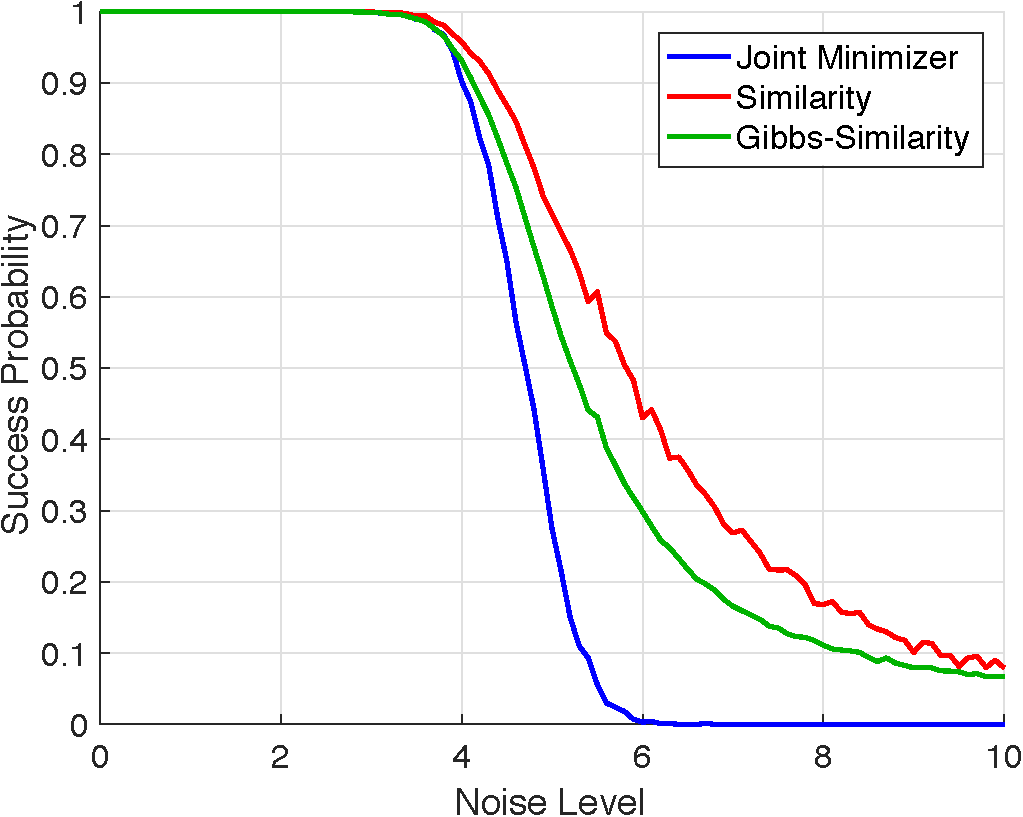
\includegraphics[width=\linewidth]{figures/ch_generic_approach/gnm_g50_b950_gibbs}
      \caption{$5\%$ of solutions are \good.}
      \label{fig:gnm_5_gibbs}
  \end{subfigure}
  \hfill
  \begin{subfigure}[b]{.49\textwidth}
      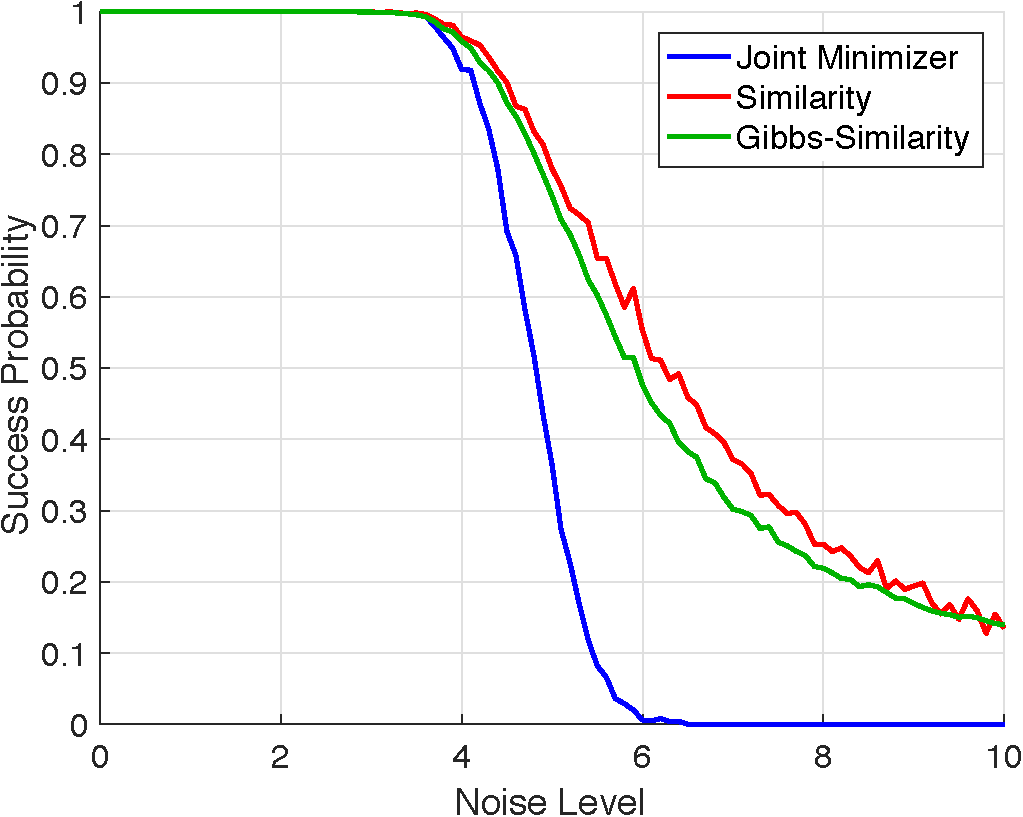
\includegraphics[width=\linewidth]{figures/ch_generic_approach/gnm_g100_b900_gibbs}
      \caption{$10\%$ of solutions are \good.}
      \label{fig:gnm_10_gibbs}
  \end{subfigure}
  \\[.5cm]
  \caption{Gibbs relaxation shows almost the same performance. Experimental
    results where $5\%$ \textbf{(a)} and $10\%$ \textbf{(b)}. Model and setting
    are the same as in Section~\ref{sec:proof_of_concept}.}
  \label{fig:gnm_gibbs}
\end{figure}

Since the Gibbs relaxation chooses every solution $c \in \mathcal{C}$ with a probability
proportional to $w^G_{\beta^*}(c, X')\cdot w^G_{\beta^*}(c, X'')$, we define its
success probability as
\begin{equation}
  P_\mathscr{A}^G(X',X'')
    \coloneqq \frac{\sum_{c \in \sgood} w^G_{\beta^*}(c, X')\cdot w^G_{\beta^*}(c, X'')}
      {\sum_{c \in \mathcal{C}} w^G_{\beta^*}(c, X')\cdot w^G_{\beta^*}(c, X'')}
\end{equation}
where $\beta^*$ is the value $\beta$ that
maximizes~(\ref{eq:gibbs_similarity_maximization_objective}). Notice that the
sums in the numerator and denominator are computed over different sets of
solutions. Notice that this formula is a full analogy
of~\eqref{eq:uncert:prob_succ}.

Figure~\ref{fig:gnm_gibbs} shows, under the same setting as in
Section~\ref{sec:proof_of_concept}, that the Gibbs relaxation provides yields
almost the same performance and thus can be considered as a viable variant
of the approximation set-based approach. This idea will be massively exploited 
in Chapter~\ref{ch:free_energy}.

\section{Discussion and Conclusion}
\label{sec:gen_appch_conclusion}

In this chapter, we introduced an approximation set-based approach to robust
optimization and justified it via a so-called Approximation Set Coding which
provides an information-theoretic background. Below, we will elaborate on some
points which are, in our view, highlighting its most interesting and/or
controversial properties.

\subsection*{Role of the logarithm}

Consider the comparison between the empirical ASC score~\eqref{eq:asc_mutual_information_formula}
\begin{equation*}
  \log 
    \frac{|\mathbb{\C}| \; |\Delta \mathcal{C}_\gamma(X', X'')|}%
      {|\mathcal{C}_\gamma(X')| \; |\mathcal{C}_\gamma(X'')|}
\end{equation*}
and the empirical similarity score~\eqref{eq:simple}:
\begin{equation*}
  \frac{|\mathcal{C}||{\mathcal{C}_\gamma}(X') \cap {\mathcal{C}_\gamma}(X'')|}
    {|{\mathcal{C}_\gamma}(X')||{\mathcal{C}_\gamma}(X'')|}.
\end{equation*}
Note that there is a difference in putting the logarithm in front of the 
ASC score. Although both have their maxima at the same $\gamma$, this logarithm
will be of essential importance later in Chapter~\ref{ch:free_energy} so
it is instructive to explain this difference.

The numerator and the denominator of the score can be seen as the
alternative and the null hypothesis, respectively, in statistical hypothesis
testing~--- the likelihood ratio test. One can view the usage of logarithm of
the likelihood ratio as a tool for ensuring asymptotic normality of estimators
in the case of weak coupling. For the main objective of this chapter, using the
logarithm had no special implications, since we were interested in the $\gamma^*$
which maximized score, but not in the score itself.

We should also note that the coding argument which we brought when deriving ASC
implies that logarithm allows to quantify the informativeness/capacity using \textit{bits}
(or \textit{nats}, depending on the type of the logarithm in use). This is 
turns the ASC score into the one which allows interpretable value~--- i.e. the one
answering ``how many bits of information can the model extract''.
\index{Nat (measure of information)}

\subsection*{Is the way of defining approximation unique?}
As one can see from the material of this chapter, the whole approximation
set-based approach rests on \textit{some notion} of closeness of the given
solution to the optimal one ($c^\bot$). We quantified this notion in terms of
parameters $\gamma$ or (in case of Gibbs approximation) $\beta$. But there
exists a whole zoo of other possible parametrizations, for example,
parametrizing by the step $t$ of a stepwise algorithm. However, we advocate the
point of view that such parametrization should yield a local topology around
each solution according to the following informal procedure:

\begin{enumerate}
  \item define certain measure of local closeness of solutions around the optimal;

  \item make an assumption: each solution \textit{is} the optimal solution for some
  input;

  \item local approximation topologies induced by the above create a ``cover''
  of the whole solution space; 
  \index{Topology}
  \index{Local approximation topology}

  \item derive conditions under which such a covering by local topology is can be
  turned into metric space (metrization theorems); \index{Metrization theorems}

  \item the above allows to create a uniform (i.e. non-local) closeness relation.
\end{enumerate}
This high-level roadmap gives some insight into the final goal of such a journey:
understand the structure of solution space in a problem-specific manner.

\subsection*{Are all solutions in the intersection created equal?}
Our method expects all solutions in the best approximation set intersection to
be equally desirable (e.g., equally good for a third, unknown instance). In some
cases, it might be useful to choose the solution based on some problem specific
criterion, e.g., choose the solution closest to the centroid of the intersection
set.

\subsection*{Will more input lead to better results?}
We mostly studied the two instance scenario because this is the minimum number
of instances necessary  to distinguish information from noise. Often, however,
more than two instances are available. The extension to multiple instances is
not immediately obvious.

There are several ways of addressing it: (a) first, one can break it into pairs
and average. This is how the framework is intended to be used in practice; (b)
second, one can derive a version of ASC for multiple agents. The latter approach
sounds much more interesting from the research prospective, as it is not clear
what would be the channel analogy in case of several agents (remember, in the
two instance scenario, we considered one data point as a codebook benchmark, and
the other as error problem generator). On can as well go in the direction of a
straightforward generalization of the similarity
formula~\eqref{eq:asc_mutual_information_formula}. In the course of our
research, some attempts have been made in that direction and they yielded
promising results.


\subsection*{Can we find efficient algorithmic solutions?}

The remark after Theorems~\ref{thm:simple}--\ref{thm:worst_case} tells that one
of the pitfalls of approximation set-based approach consists in computation of
the similarity score. While we used brute-force enumeration for our
proof-of-concept experiments, it would be of a great importance to find either
(a) analytical estimations for the similarity score or (b) efficient algorithms
for computing it.

In this chapter, we tackled case (a) and made an attempt to derive a very simple
analytical estimator, which uses the knowledge of the true distributions. This
assumption, of course, renders it useless in real cases, but allows usage of
plug-in estimators of the true distributions.

On a much higher level which uses less information about the true distributions,
the approach (a) will be tackled in Chapter~\ref{ch:free_energy}.

In specific cases, such as application to combinatorial algorithms, the approach
(b) can be used by utilizing combinatorial structure of the solutions. This will
be shown in Chapter~\ref{ch:mst}.

\subsection*{Similarity as a computational goal-specific measure}
An interesting side-result that we did not focus on in this chapter is the
expressiveness of instance similarity $S_{\gamma^*}$. In fact, it utilizes a
\textit{computational goal-induced} topology on the set of solutions. We bring
here a motivation which was best described in~\citep{jcss:2017}.
\index{Topology}
\index{Computational goal-induced topology}
For example, consider the problem of computing a shortest path between two given
vertices in a graph $G$. 
%
Having two instances $X'$ and $X''$ of this problem, one may attempt to measure
the similarity of these instances using certain structural information exposed to
us~--- e.g.,~the correlation coefficient or the Euclidean distance between the
vectors containing the edge weights.
\index{Euclidean distance}

However, if the instances differ a lot only in some weights which are usually
high and thus these edges that are never used in any nearly-shortest path, then
the similarity approach will correctly consider such examples as similar,
whereas for example the correlation coefficient will tell the opposite.
%
At the same time, if the computational goal was a maximum matching of edges
rather than the minimizing the weight cost, the similarity would regard the two
instances as significantly different.
%
This example highlights the need for a measure of \emph{similarity of instances
with respect to a computational goal}. This is performed by inducing a local topology
around each solution, and this topology depends only on the computational goal
and not on anything else.

